% !TeX encoding = UTF-8
% !TeX program = xelatex
% !TeX spellcheck = en_US

\documentclass[degree=master, degree-type=professional, output=electronic, fontset=windows]{ustcthesis}
% degree      = doctor | master | bachelor
% degree-type = academic | professional
% language    = chinese | english
% fontset     = windows | mac | ubuntu | fandol

% 加载宏包、全部的配置
% !TeX root = ./main.tex

\ustcsetup{
  title              = {轻量级仿真平台硬件平台建模及应用的设计与实现},
  title*             = {Design and implementation of hardware platform modeling and application of lightweight simulation platform},
  author             = { },
  author*            = { },
  speciality         = { },
  speciality*        = { },
  supervisor         = { },
  advisor            = { },
  supervisor*        = { },
  advisor*           = { },
  % date               = {2017-05-01},  % 默认为今日
  professional-type  = {专业学位类型},
  professional-type* = {Professional degree type},
  % department         = {数学科学学院},  % 院系,本科生需要填写
  % student-id         = {PB11001000},  % 学号,本科生需要填写
  % secret-level       = {秘密},     % 绝密|机密|秘密|控阅,注释本行则公开
  % secret-level*      = {Secret},  % Top secret | Highly secret | Secret
  % secret-year        = {10},      % 保密/控阅期限
  %
  % 数学字体
  % math-style         = GB,  % 可选:GB, TeX, ISO
  math-font          = xits,  % 可选:stix, xits, libertinus
}


% 加载宏包

% 定理类环境宏包
\usepackage{amsthm}

% 插图
\usepackage{graphicx}

% 三线表
\usepackage{booktabs}

% 跨页表格
\usepackage{longtable}

% 算法
\usepackage[ruled,linesnumbered]{algorithm2e}

% SI 量和单位
\usepackage{siunitx}

\usepackage{enumerate}

% 参考文献使用 BibTeX + natbib 宏包
% 顺序编码制
\usepackage[sort]{natbib}
\bibliographystyle{ustcthesis-numerical}

% 著者-出版年制
% \usepackage{natbib}
% \bibliographystyle{ustcthesis-authoryear}

% 本科生参考文献的著录格式
% \usepackage[sort]{natbib}
% \bibliographystyle{ustcthesis-bachelor}

% 参考文献使用 BibLaTeX 宏包
% \usepackage[style=ustcthesis-numeric]{biblatex}
% \usepackage[bibstyle=ustcthesis-numeric,citestyle=ustcthesis-inline]{biblatex}
% \usepackage[style=ustcthesis-authoryear]{biblatex}
% \usepackage[style=ustcthesis-bachelor]{biblatex}
% 声明 BibLaTeX 的数据库
% \addbibresource{bib/ustc.bib}

% 配置图片的默认目录
\graphicspath{{figures/}}

% 数学命令
\makeatletter
\newcommand\dif{%  % 微分符号
  \mathop{}\!%
  \ifustc@math@style@TeX
    d%
  \else
    \mathrm{d}%
  \fi
}
\makeatother
\newcommand\eu{{\symup{e}}}
\newcommand\iu{{\symup{i}}}

% 用于写文档的命令
\DeclareRobustCommand\cs[1]{\texttt{\char`\\#1}}
\DeclareRobustCommand\pkg{\textsf}
\DeclareRobustCommand\file{\nolinkurl}

% hyperref 宏包在最后调用
\usepackage{hyperref}



\begin{document}

% 研究生论文:
%   封面,原创性声明和授权使用声明
%   frontmatter: 摘要,目录,[图、表清单],[符号说明]
%   mainmatter: 正文章节,参考文献
%   appendix: 附录
%   backmatter: 致谢,已发表论文列表
%
% 本科生论文:
%   封面
%   frontmatter: 致谢,目录,摘要
%   mainmatter: 正文章节,参考文献
%   appendix: 附录

\maketitle
\copyrightpage

\frontmatter
% !TeX root = ../main.tex

\ustcsetup{
  keywords = {
    电子系统级设计, 轻量级仿真平台, SimPy, 多目标优化, 设计空间探索,硬件平台建模
  },
  keywords* = {
    Electronic System Level,Lightweight simulation platform, SimPy, Multi-objective optimization, Design Space Exploration,Hardware platform modeling
  },
}

\begin{abstract}
  随着片上系统(SoC,System on Chip)的设计复杂性不断提高,在设计前期通过对系统层次进行软、硬件的划分
  对片上系统各方面性能的影响日趋增加,迫切需要高效快捷的性能分析和验证方法学。
  而ESL(Electronic System Level)设计方法不仅提供快速的仿真验证方法,还提供了
  详细的性能分析指标,现如今已经成为SoC设计领域最先进的设计方
  法。为缩短芯片设计周期,设计者需要在设计前期快速找到一种满足设计要求的最佳
  参数配置。设计空间探索(Design Space Exploration,DSE)就是通过在大量不同的
  参数配置下执行仿真,从而实现上述目标的过程。现有的仿真验证平台无法进行快速的仿真
  验证,而设计空间探索流程中需要进行仿真的快速迭代。因此需要实现一个能够快速进行仿真验证的
  轻量级仿真平台。

  本论文主要是通过ESL设计方法设计并实现一个基于SimPy仿真引擎的仿真验证平台,并基于该仿真
  平台实现设计空间探索流程。该仿真平台能够快速地进行仿真验证并输出设计空间探索所需要的
  目标参数。
  本文的主要工作如下:

  \begin{enumerate}
    \item 设计并实现了轻量级仿真平台中硬件平台模块,包括硬件平台构建模块以及硬件模型建模。与仿真平台
    软件部分以及总线互联模块共同组成整个轻量级仿真平台,以用例文件
    和硬件配置文件作为输入,完成业务仿真整个流程,并最终输出仿真结果以及存
    储仿真过程中信息的数据库文件,提高了业务仿真的效率。
    \item 设计并实现设计空间探索流程中的训练集生成模块以及仿真平台预测模型,参与实现了多目标的
    设计空间探索,得到了最终的帕累托最优解集。并通过对最优解集进行验证和分析,得出芯片的最优设计方案。
  \end{enumerate}

  本文详细介绍了包含轻量级仿真平台硬件平台建模和设计空间探索流程中训练集生成模块以及仿真平台预测模型的需求分析、概要设计、系统设计与实现和系统测试与结果分析。
  并且为业内在前期芯片架构方案设计阶段提供新的一整套解决方案,并设计并实现了一个轻量级仿真平台,为一些快速的设计方案的实
  现提供了更加方便的平台。
\end{abstract}

\begin{abstract*}
  With the increasing design complexity of system on chip (SOC), the impact on all 
  aspects of system on chip performance is increasing through the division of 
  software and hardware at the system level in the early stage of design. There 
  is an urgent need for efficient and fast performance analysis and verification 
  methodology. ESL (electronic system level) design method not only provides 
  fast simulation verification method, but also provides detailed performance 
  analysis indicators. Now it has become the most advanced design method in 
  the field of SoC design. In order to shorten the design cycle of microprocessor, 
  designers must quickly find an optimal parameter configuration to meet the 
  design requirements in the early stage of design. Design space exploration (DSE) 
  is a process to achieve the above objectives by performing simulation under a 
  large number of different parameter configurations.The existing simulation 
  verification platform can not carry out fast simulation verification, 
  but the rapid iteration of simulation is needed in the process of design 
  space exploration. Therefore, it is necessary to implement a lightweight 
  simulation platform that can quickly carry out simulation verification.

  This paper mainly designs and implements a simulation verification platform based on simpy simulation engine through ESL design method, and realizes the opening of design space exploration process based on the simulation platform. The simulation platform can quickly carry out simulation verification and output the target parameters required for design space exploration.this article has done the following parts:

  \begin{enumerate}
    \item Design and implement a hardware platform module in the lightweight simulation platform, including hardware platform construction module and hardware model modeling. Together with the software part of the simulation platform and the bus interconnection module, it forms the whole lightweight simulation platform, takes the use case file and hardware configuration file as the input, completes the whole process of business simulation, and finally outputs the simulation results and the database file storing the information in the simulation process, which improves the efficiency of business simulation.
    \item Design and implement the training set generation module and simulation platform prediction model in the design space exploration process, participate in the multi-objective design space exploration, and obtain the final Pareto optimal solution.Through the verification and analysis of the optimal solution set, the optimal design scheme of the chip is obtained.
  \end{enumerate}

  This paper introduces in detail the demand analysis, outline design, system design and implementation, system test and result analysis of the training set generation module and simulation platform prediction model in the process of hardware platform modeling and design space exploration of lightweight simulation platform. This 
  article provides a new set of solutions for the industry in the pre-chip architecture design stage, and designs and implements 
  a lightweight simulation platform, which provides a more convenient platform for the realization of some rapid design solutions.

\end{abstract*}

\tableofcontents
\listoffigures
\listoftables

\mainmatter
% !TeX root = ../main.tex

\chapter{绪论}

\section{选题意义及选题背景}
随着片上系统(System on Chip,SoC)的发展,越来越多的微处理器和芯片被嵌入到一个
芯片上,导致片上系统的设计复杂性不断提高。在上市时间迅速减少以及功耗降低的需求背景下,
较低抽象层次的RTL设计不能满足SoC设计的需求。现已将设计抽象推向电子系统级别(Electronic System Level,ESL),
能够在SoC设计过程中进行快速原型设计和早期验证\cite{1},或在设计过程能够通过在设计初期能高效迭代探索出比较
准确的设计方向或大致几种比较优秀的方案就显得尤为重要。如果在芯片的RTL设计和验证过程中才发现架构或
软硬件划分无法满足系统功能、性能和成本的要求,就会导致大量的重复工作。ESL设计能够提供比RTL设计更快的仿真速度,
以及根据实际需求所要求的不同抽象层次的时序精度, 以进行SoC系统整体性能的评估。软硬件协同设计采用统一的语言描述
系统功能,可以在实现系统前对整个系统进行仿真,以便于及早发现功能问题。接着根据整个系统的约束对系统进行
硬件划分。然后软件和硬件部分可以同步开发,最后再一起协同验证。采用软硬件协同设计可以大大缩短芯片的开发
周期,并提高芯片性能,降低成本。现如今软硬件协同设计的基本思路如图1.1所示:
\begin{figure}
    \centering
    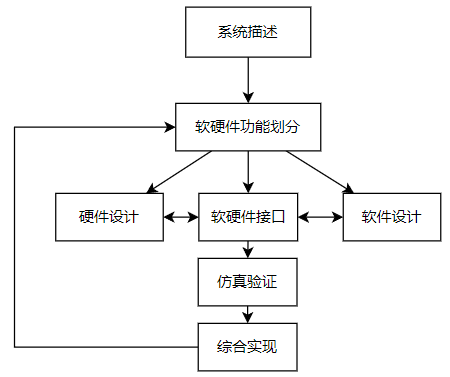
\includegraphics[width=0.5\textwidth]{软硬件协同设计基本思路.png}
    \caption{软硬件协同设计的基本思路}
    \label{fig:badge}
\end{figure}

仿真模型模型的建立和验证是处理器设计周期中一个重要阶段。当前,大多数的处理器仿真模型为C/C++所写,仿
真模型的建立基于SystemC\cite{2}编写,用于统一硬件模型设计以及上层软件平台,这虽然节省了一定的沟通成本,以及
保持体系结构设计及验证阶段模型的一致性。但灵活性较差,为了追求验证结果的精度,系统复杂度较大。因此,
为了较快的完成架构空间探索,我们需要重新设计一个轻量级,且灵活可配置的仿真平台。

在硬件/软件协同设计过程\cite{3}中提高设计生产率的趋势之一是提高抽象水平。如今,大多数设计流程的实现过程都是基
于寄存器传输级别(RTL)的描述。一方面,用于仿真的语言(例如SystemC)提供了更高的抽象级别,另一方面,
通过高层次合成(High Level Synthesis,HLS)\cite{4}的能力也提供了更高的抽象级别。高级综合的目的是双重的。首先,通过在更高层次上描述系
统,可以获得生产率的提高。其次,由于设计转换发生在更高的层次上,因此有更大的探索设计空间的潜力,这将导
致更好的设计。这种发展的重要性直接影响到设计成本。

较大的设计空间、较高的性能目标要求以及紧迫的上市时间要求对系统的设计提出了极大的挑战。通常,设计空间探
索 (DSE)\cite{5} 在早期开发阶段执行,以在满足整体系统设计要求的多个高级设计配置之间进行选择。自动的设计空间中
寻找和探索可行的解决方案。

本仿真设计平台基于Python的Simpy\cite{6}包构建的仿真环境。Python语言具有简易快速的特点,我们可以快速的重构整个
仿真平台。同时基于这种仿真环境构建的仿真平台具有仿真速度快的优点,我们在设计空间探索过程中可以快速进行,
满足设计空间探索的要求。在本文中我们打通了在极大的设计空间中探索能使得系统性能最优的设计参数的设计空间
探索流程。

\section{国内外研究现状及发展趋势}

\subsection{仿真建模技术的发展现状}
随着片上系统系统的复杂度不断提升,高层建模技术由于其更快的建模速度、更短的仿真时间
以及更高的抽象程度逐渐被大多数研发水平高的机构、高校、电子设计自动化(Electronic Design 
Automation,EDA)公司所重视,并开发出多种高水平的仿真模拟工具以及仿真平台,具有代表
性的有Synopsys的CoWare,Mentor的Vista,Carbon的SoC Designer等等。这些工具提供了许多芯片设计
过程中遇到问题的解决方案,从各模块模型的建立、系统架构的分析到功能验证以及时序分析,进一步
分析功耗以及时延等性能指标\cite{38},甚至给出了高层次综合(High Level Synthesis,HLS)方案。

ESL设计作为系统级设计方法,其核心的思想是从算法级模型转变过来的。ESL设计方法学和ESL设计工具
最早是在20世纪90年代提出的。随着SoC设计技术的发展,ESL设计逐渐受到重视,真正能够执行设计
流程的ESL设计工具这些年才出现。ESL设计现在已经发展成系统软硬件设计、协同验证的一种方法学。
ESL设计是以抽象方式来描述SoC系统,给软硬件工程师提供一个虚拟的硬件原型平台,用于进行硬件系统
结构的探察以及软件程序的开发。

现如今硬件建模仿真平台一部分基于C/C++编写,只能进行串行或多线程仿真和验证,后期的硬件原型模型建立需要采
用Verilog等硬件描述语言完成。另外一部分用SystemC完成,SystemC\cite{7}是一种系统级建模语言,
在C++语言的基础上扩展了一系列的硬件库。SystemC更擅长描述
复杂的算法和控制流程,可以更清楚的描述出整个电子系统的复杂行为。SystemC由Accellera定义和推广,SystemC
适用于系统级建模、体系结构探索、性能建模、软件开发功能验证和高级综合,通常和电子系统级设计和事务级建模(TLM,Transaction Level Modeling)
相关联。SystemC语言既能按照硬件设计的要求进行时钟精
确的并行设计,也可以按照软件设计人员的要求进行抽象层级较高的串行设计,还能兼容C语言
、C++语言,且有专门的标准接口处理SystemC语言与硬件语言的连接问题,因此很适合作为桥梁
连接软件设计和硬件设计\cite{37}。SystemC可以在系统级用高级语言同时描述软件
行为和硬件行为,实现软硬件协同设计\cite{40}。图1.2是基于SystemC的软硬件协同设计流程图。

\begin{figure}
    \centering
    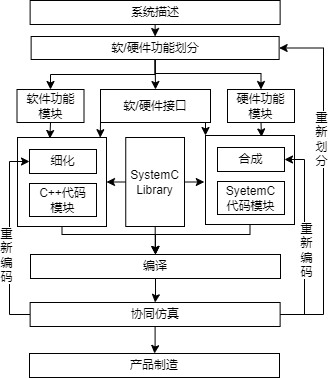
\includegraphics[width=0.5\textwidth]{SystemC软硬件协同设计流程图.png}
    \caption{基于SystemC的软硬件协同设计流程图}
    \label{fig:badge}
\end{figure}

基于SystemC的实现方式相对于前者的优点是仿真平台的建立以及后期硬件模型验证统一起来,能够加快开发流程,节约设计
流程和设计成本。在架构探索阶段,通过对简易建模的仿真分析。得出适合设计要求的架构设计,并在该架构上快速仿真以
得出影响系统性能的因素。在功能验证方面,采用SystemC事务级模型对SoC高层模型进行设计和验证\cite{8}。基于SystemC的标准
事务级建模支持不同系统之间的模型交换。电子系统级设计抽象的描述系统级芯片的行为,能在芯片设计的前期就满足深入
设计芯片系统仿真的需求\cite{9}。这已经成为SoC设计领域前沿的设计方法。

现在又提出了新的仿真工具Simpy,SimPy最初基于Simula和Simscript的思想,但使用标准的Python。它结合了两个以前
的软件包,即Simula风格的SiPy和Simscript风格的SimPy。SimPy 是一个基于标准 Python 以进程为基础的离散事件仿真
框架。SimPy 中的进程是由 Python 生成器构成,生成器的特性可以模拟具有主动性的物件。但现在Simpy很少用于大型平台
建模,主要用于某个具体场景仿真建模即单场景仿真\cite{10},如使用SimPy仿真框架进行基于森林的供应链建模\cite{11}。
\subsection{芯片系统性能分析发展现状}
现如今对于芯片性能进行评估主要从两个方面进行:第一种方法是使用仿真器,如Worm\_sim、NoCSim
、NIRGAM等等。还有一个方法是建立分析模型,如基于排队论或链路拆解原理的分析模型\cite{39}。
前者由于非定制的原因仿真精度不足但仿真速度较快,后者仿真精度高但速度较慢。
现在已经有了能应用于CPU等复杂SoC的仿真工具,如应用广泛的Gem5\cite{12}。它由研究机构和企业合作发展
既支持应用程序仿真又支持全系统仿真,时钟周期准确,可配置并集成工业化标准结构和CPU模型。
\subsection{设计空间探索流程的发展现状}
设计空间探索是指根据系统设计所关心的参数而对不需要的参数进行系统分析和修剪\cite{13},虽然DSE适用于所有类型的系统,但主要
涉及到的还是电子和嵌入式系统。现代嵌入式系统通常具有异构的多处理器系统架构。他们由处理器组成,从完全可编程的内核
到针对时间紧迫任务需求的完全专用的硬件模块。此类系统的组件越来越也多的集成到单个芯片上,从而产生了异构的多处理器
片上系统(MPSoC)架构\cite{14}。为了应对此类系统的复杂性,近15至20年来,电子系统级设计方法这种新设计方法随之出现。并用此
建立里一些高级模型,使建模工作最小化,并对执行速度进行了优化。在此基础上,我们能够在非常早期的设计阶段就应用设计
空间探索。在此探索阶段,可以探索各种不同的设计替代方案。但设计空间探索的过程也极具挑战性,因为探索的设计空间很大。
例如,用于探索应用程序到处理资源的不同映射\cite{15}以及不同调度策略及系统参数对系统性能的影响。

\section{本论文的主要工作}
本文详尽的阐述了一个基于Simpy仿真环境搭建的仿真平台中硬件平台的构建、硬件模型
的建模以及基于这个仿真平台实现的设计空间探索流程。该仿真平台能够快速的让用例在
硬件平台上运行并给出仿真结果及仿真运行过程中的任务执行细节以及硬件资源的利用情
况,打通了设计空间探索的流程,并最终给出设计参数集合的帕累托最优解集。本文将从
以下几个方面进行阐述:

\begin{enumerate}
    \item 仿真平台硬件模块的整体架构设计,主要包括硬件平台配置文件的读取以及根据硬件配置信息实例化硬件IP模型,以及用例文件
    的任务信息的读取及整合,为整个仿真平台的运行打下基础。
    \item 仿真平台Processor模块的整体架构设计,主要是各个硬件模块执行任务的逻辑以及硬件模块的实现,还包括了整个系统中交互
    的基础模型GeneralFifo的实现。
    \item 仿真平台Memory模块的整体架构设计,主要是数据在Memory模块上的读取和存储的逻辑实现,以及Memory模块与总线互联模块的
    交互设计。
    \item 设计空间探索流程的实现,主要包括基于仿真平台实现仿真过程的预测模型,并基于预测模型实现设计空间探索流程,最终给出帕
    累托最优解集,并对设计空间探索结果进行分析。
\end{enumerate}

在整个项目过程中,本人的主要工作如下:

\begin{enumerate}
    \item 设计并实现基于Simpy的仿真平台,完成仿真平台设计中的硬件平台构建模块、
    Processor模块、Memory模块、数据库模块以及整个仿真平台各个模块之间的交互部分。
    \item 根据仿真平台实现预测模型,并基于硬件模块实现设计空间探索流程,并根据最
    终给出的帕累托最优解集给出相应的结果分析。
\end{enumerate}

\section{本文的组织结构}
本文主要分为7个章节,每个章节的具体内容安排如下:

第一章:绪论:介绍不同模型仿真及系统仿真的发展,以及设计空间探索的国内外发展现状,并介绍了本文的研究内容。

第二章:相关技术介绍:对仿真平台及设计空间探索的设计实现所用到的关键技术进行详细的阐述,一方面介绍了系统建模的基础知识
以及我们所采用的仿真环境Simpy框架,另一方面介绍了仿真平台的整体流程以及相关模块的整体设计。

第三章:需求分析:基于仿真平台的功能及性能需求及设计空间探索结果分析准确性的需求的基础上,对仿真平台及设计空间探索的需求
分析进行详细的阐述。

第四章:概要设计:这部分主要是在需求分析的基础上对轻量级仿真平台中硬件平台建模的设计及设计空间探索模块的设计进行简要的阐述,对仿真平台的
整体架构及各个模块的功能划分进行了详细的说明。通过概要设计,为整个应用的实现做好铺垫。

第五章:详细设计与实现:基于概要设计的方案,结合软件工程的的开发思想,详细的介绍了仿真平台硬件平台的搭建、各个硬件模型的
建模、整个用例任务的执行、设计并实现了各个硬件模块之间数据及消息交互相应的接口、设计空间探索流程的具体实现。同时,我们对
设计空间探索流程最终给出的设计参数的集合进行了分析并给出相应的结论。

第六章:系统测试及结果分析:在实现了仿真平台及设计空间探索流程之后,我们基于仿真平台的执行以及结果准确性等方面对整个仿真平
台进行了测试,确保仿真平台能达到预期的结果。

第七章:总结和展望:在本章,笔者对这篇论文进行简单的总结,并对仿真平台及设计空间探索流程中的不足进行了描述,并对仿真平台及
设计空间探索流程提出了未来的展望。


% !TeX root = ../main.tex

\chapter{相关技术简介}
本章简要介绍与本文密切相关的几种技术及框架,整个系统基于这几种技术
进行开发。在本章,我们将对ESL建模、Simpy仿真框架
以及一些相关技术进行详尽的阐述。

\section{ESL建模介绍}
ESL(Electronic System Level)设计和验证方法是一种电子设计方法。基本方法是
使用高级语言或使用图形化工具对整个系统的行为进行建模。在新的语言不断出现的情况下,
现在常常使用SystemC来作为一种抽象的建模语言。

ESL是许多世界领先的片上系统设计公司的既定方法,并且现在更多地用
于系统设计。ESL最初是被使用为一种“无实现链接”的算法建模方法,现在正
在逐渐变成一套互补的方法,支持嵌入式系统的设计、验证和调试,一直到定
制SoC的硬件和软件实现\cite{41}。ESL设计流程图\cite{42}如图2.1所示。

\begin{figure}
  \centering
  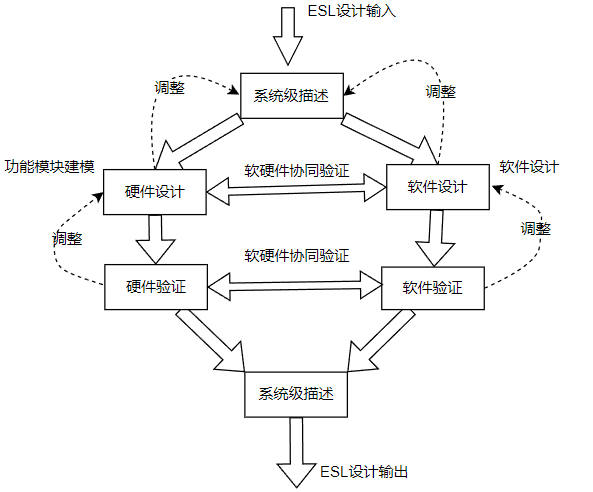
\includegraphics[width=0.7\textwidth]{ESL设计流程图.png}
  \caption{ESL设计流程图}
  \label{fig:badge}
\end{figure}

\section{SimPy仿真框架介绍}
SimPy是一个基于标准Python的基于过程的离散事件仿真框架。它的事件
调度机制基于Python的生成器Generator来实现的,可用于异步网络或者用来实现多代理系统(具有
模拟和真实通信)。

SimPy中的进程是由Python中的生成器函数来定义的。所有的进程都存在于一个仿真
环境中。它们通过事件机制与仿真环境来彼此交互。在它们的生命周期中,它们会创建
事件并创建yield语句以等待进程被触发。当一个进程产生一个事件时,该进程被挂起。
SimPy中的进程在事件发生时被触发(我们说事件被触发)。多个进程可以等待同一个事件。
SimPy通过记录它们创建并等待该事件的顺序,并以相同顺序恢复这些进程。同时,SimPy中一个重要的事件类型
为Timeout,此类事件在一定量的(模拟)时间后触发。 它们使仿真环境中的进程在
给定的时间内休眠(或保持其状态)。所有事件都可以调用Environment进程所在的的
方法来创建。

SimPy提供了三种类型的容器,可用于同步进程或对拥塞点进行建模。第一种为resource,
支持优先级和抢占的共享资源;第二种为container,用于在过程之间共享同种类物质的资源,
无论该种类资源是连续的还是离散的;第三种为store,用于存储支持特定对象请求的可能无限数量的对
象的共享资源。此外,我们还可以自定义资源类型的实现。

  \section{多目标优化介绍}
  在我们对芯片架构进行设计空间探索的过程中,系统架构的目标参数通常都不止一个。在多目标优化问题中,
  多个目标参数之间可能会存在冲突,并且可能不能同时达到最优。以遗传算法为代表的许多进化算法\cite{20},
  都具有能够生成多个点并且能向多个方向进行搜索的特点,因此十分适合这种求解的最优解所在的搜索空间非常
  复杂的多目标优化问题\cite{21}。

  多目标优化问题是在给定约束条件的前提下,求多个目标函数的最大或最小的问题\cite{22}。在多个目标函数中,有
  的可能是最小化目标函数,有的可能是最大化目标函数。多个目标之间可能会拥有不同的单位,也可能在优
  化某个目标时损害其他目标。但这并不意味着多目标优化问题可能没有最优解,事实上是可以有的,为了求
  出比较合理的解,这里引入多目标优化问题的合理解集——Pareto最优解\cite{23}。

  在解决单目标优化问题的时候,这一类问题一定有唯一的最优解,但当解决多目标优化
  问题的时候,多个目标之间可能互相影响,所以最优解有可能不止一个。所以多目标问
  题的最优解有如下定义:

  给定一个多目标优化问题minf(x),设X*属于Ω,如果不存在X属于Ω,使得满足以下条件:对于f(x)的任意子目标函数
  fi(x)都有fi(X)≤fi(X*),同时至少存在一个子目标函数fi(x)使得fi(X)< fi(X*)那么,我们称X*是一个
  强Pareto最优解\cite{24}。

  \section{SQLite数据库介绍}
  SQLite因为其小巧、方便使用以及符合ACID事务特性的优点而受到开发人员的广泛喜爱,它是目前使用最多的
  小型数据库之一\cite{25}。SQLite由D. Richard Hipp设计开发。在编写导弹驱逐舰上运行的设备控制程序的时候
  ,他产生了设计SQLite的想法\cite{26}。SQLite支持当今几乎所有的主流操作系统,如Android、IOS和Windows等
  ,还能在Python、Java、C\#等语言下使用,同时也支持ODBC接口。相比于传统数据库如MySQL、PostgreSQL 
  等,SQLite对于数据的处理速度要更加迅速\cite{27},而且它运行时只需要占用非常低的资源,通常只占用几百K的计算机
  内存,因此被许多嵌入式产品所采用。

  \section{仿真平台整体介绍}
  整个轻量级仿真平台由整个一起完成,为了更好的介绍设计实现
  的硬件平台相关的模块和了解仿真平台进行业务的整体流程,接下来主要介
  绍下仿真平台的整体架构、业务仿真进行的流程以及业务仿真在其他模块上的执行。

\subsection{仿真平台整体架构}
轻量级仿真平台建模整体分为硬件平台模块建模以及软件平台模块。硬件平台模块分为:Processor模块、总线互联模块
以及Memory模块;软件平台模块主要分为:输入处理模块以及调度器模块。仿真平台功能模块示意图如图2.2所示:

\begin{figure}
  \centering
  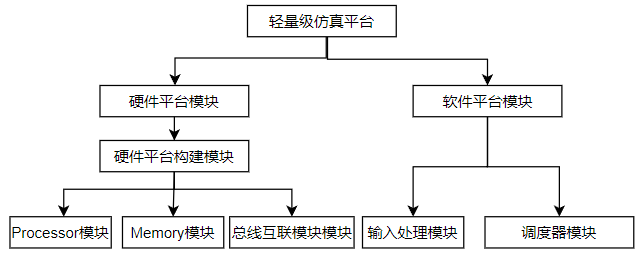
\includegraphics[width=1\textwidth]{仿真平台功能示意图.png}
  \caption{仿真平台功能模块示意图}
  \label{fig:badge}
\end{figure}

\subsection{仿真平台业务仿真流程}
仿真平台的实现是为了在芯片正式生产之前对芯片系统架构以及功能进行验证,所以需要通过
真实的用例在仿真平台上执行验证。仿真平台的业务仿真流程图如图2.3所示:

\begin{figure}
  \centering
  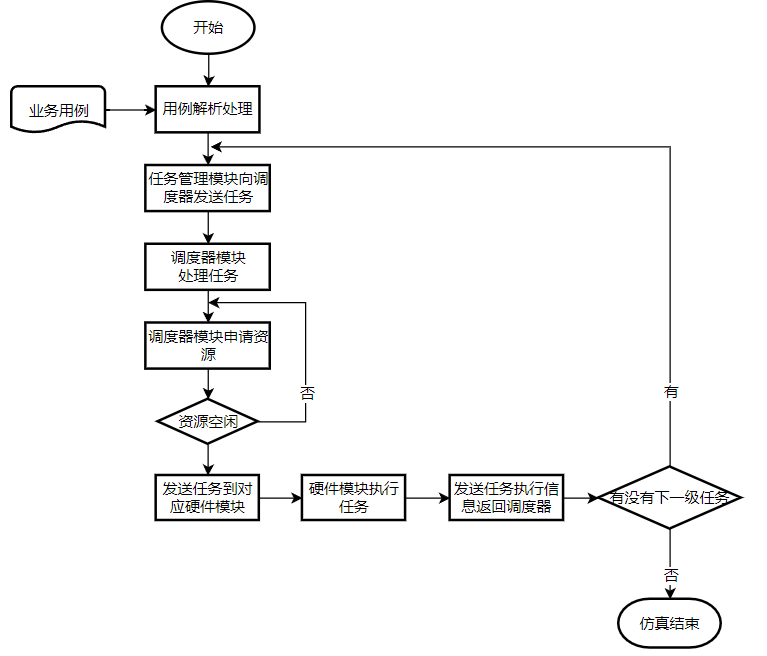
\includegraphics[width=1\textwidth]{仿真平台业务仿真流程图.png}
  \caption{仿真平台业务仿真流程图}
  \label{fig:badge}
\end{figure}

接下来简要的介绍整个业务仿真流程的执行,为了更好的理解本文后面设计的硬件平台模块,
下面着重介绍仿真平台与其有交互模块的设计原理以及功能。

轻量级仿真平台的输入任务模型是实例级别的数据流图模型,任务之
间以数据为触发关系,任务之间的触发为实时触发。当任务的输入数据
全部就绪后,该任务实例才会开始执行,一旦任务执行完毕,其输出数
据被触发搬运。整体的任务的数据流图示例图如图2.4所示。

\begin{figure}
    \centering
    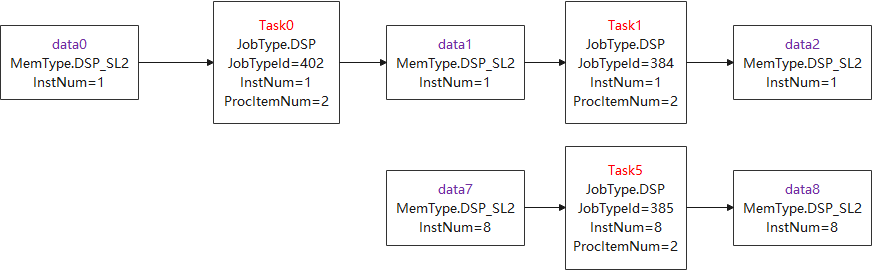
\includegraphics[width=1\textwidth]{任务数据流图示例图.png}
    \caption{任务数据流图示例图}
    \label{fig:badge}
\end{figure}

仿真平台的任务用例输入类型是描述了所有任务相关信息的
Excel文件,包括任务类型、任务执行的所属调度器、任务的
输入输出数据,数据的大小类型等等。平台初始化时通过
SaeSimulaor单实例中的load\_task\_praph方法解析任务信息
文件,并通过TaskGraphMgnt类管理。

TaskGraphMgnt类通过ExcelReader类里的方法读取输入任务用
例的Excel表,将任务信息遍历读取,根据任务用例中任务具
体信息将任务根据自身信息生成不同类型的任务对象,将数
据信息生成DataInst类对象。在Graph类中由多种类型的节
点,如图2.4任务流图示例图所示每个节点之间双向连接。
为每个TaskInst节点配置input\_data和output\_data两个字
典,为每个DataInst节点配置producer和consumer两个字典,
在Graph类中读取任务实例和数据实例,并根据在任务用例文
件中任务和数据之间关系,分别将任务实例和数据实例填入
不同节点的各自的两个字典中,并且将数据和任务之间依赖
关系作为边设为edge\_list。在读取excel的过程中构造图
的结构,并不断地将TaskInst和DataInst以及结合他们之
间的映射关系加入Graph对象中。

TaskGraphMgnt模块将所有任务全部解析并读取到Graph对象中后,当仿真系统发出
仿真执行的指令后,TaskGraphMgnt模块按照任务顺序将任务发送到调度器模块。

调度器模块负责整体任务调度,观察并接收TaskGraph Manager中就绪
任务,根据任务信息将任务分到不同子模块去分配资源,并分配到具
体硬件上去执行任务,同时接收硬件返回的response,将任务信息同
步,释放资源并触发下一级任务。调度器模块还负责管理device资源
和memory资源。调度器模块分为任务分配TOP模块、任务调度SCH模块、
资源管理RES模块几个子模块。调度模块具体结构图如图2.5所示。
  
\begin{figure}[h]
    \centering
    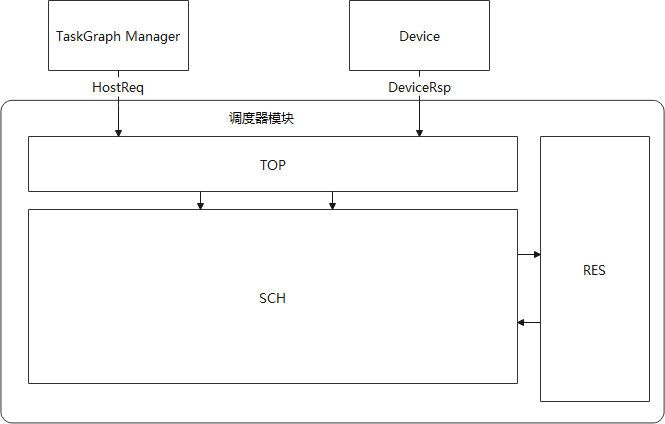
\includegraphics[width=0.8\textwidth]{调度器模块结构图.png}
    \caption{调度器模块结构图}
    \label{fig:badge}
\end{figure}
  
TOP模块负责接收任务以及硬件模型以及内部子模块发来的响应。通过
任务信息,以及响应类别,通过不同的线程将不同类别的任务分别分
到各个子模块处理。
  
SCH模块负责给任务分配资源(包括硬件模型资源CU以及硬件IP、内存
资源等等),根据任务携带的信息将任务分配给之前分配的硬件IP进
行具体的处理。
  
RES模块负责管理各个核的私有内存(包括L1D、PL2);公共内存资
源(如SL2等);管理Device资源,每个ALA支持32个Device,每个D
evice分为多个CU,CU为每个硬件模型外的任务等待队列;管理硬件
资源(如DMA、HAC等等)。其他模块通过调用这个模块的方法来申
请和释放资源。

调度器模块通过Schdule模块读取TaskGraphMgnt对象里的Graph
任务图对象读取出来。Graph对象形式是有向无环图类型,Schdule
模块先遍历有向无环图,找到DAG图中没有入度的节点即为第一个
任务或数据,将实例输入到调度器模块,由TOP模块接收判断类型,
根据信息类型转发到SCH模块。

TOP模块负责接收外部模块发送过来的任务图中实例信息以及硬件模
型处理任务完成后发送回来的响应,按照实例或者响应分开处理。
RES模块负责管理各个核的私有内存(包括L1D、PL2);公共内存
资源(如SL2等);管理Device资源。SCH模块负责向RES模块申请
管理的硬件资源和内存资源。并将任务信息或数据信息发送到申
请好的硬件IP中进行处理。

在调度器模块发送任务到具体硬件上执行后,当发生数据搬运时,
模块与模块之间的数据交互是通过总线互联模块进行的。

在仿真平台中,在不同模块之间通过总线进行通讯,而总线在不同模块上
的端口则是Port模块。针对端口设计的可扩展性,我们以Moudule Port 
Base为基础,采用Master/Slave方式。在仿真平台中,所有端口采用双
向绑定机制,即在Master端可以调用Slave端的方法.

仿真平台中现在主要有两种模块间通讯接口,一种为硬件模型模块间的接
口:Virtual Master Port和Virtual Slave Port,另一种是总线内部子
模块之间的流水线通讯接口VBusPipeLineMasterPort与VBusPipeLineSlavePort。

Master Device在硬件实例化的时候创建对应的VirtualMasterPort,
Slave Device在硬件实例化的时候创建对应的VirtualSlavePort。
Master Device一般是Processor模型,
硬件IP实例化时通过调用ProcessorBase的方法add\_port创建
Port端口。Slave Device一般是Memory模块。在平台构建
时,VirtualMasterPort和VirtualSlavePort通过硬件平台配
置表上的信息进行绑定。这两种端口都由PortMgnt进行管理,

在仿真平台硬件模块中,所有数据信息的传输都是通过总线模块进行,
所有的数据传输都是通过Port模块拆分封装成Flit格式的数据包经过
总线模块从一个硬件模块发送到另一个硬件模块。对应不同模块之间
总线模块是不可视的,能接触的只有Port,当Master设备发送数据到
对应Port上的操作如图MasterPortMgnt实现流程图所示。

\begin{figure}
  \centering
  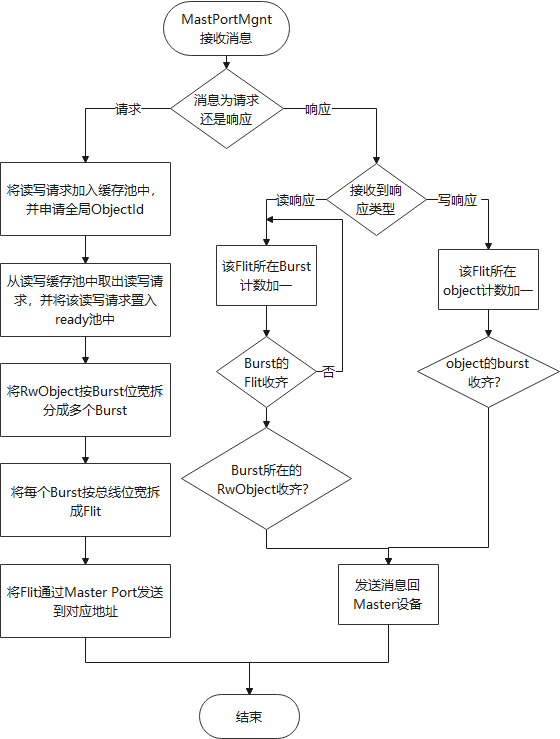
\includegraphics[width=0.7\textwidth]{MasterPortMgnt实现流程图.png}
  \caption{MasterPortMgnt实现流程图}
  \label{fig:badge}
\end{figure}

总线处理模块的主要功能是地址译码、优先级仲裁以及模拟每个
flit的传输。BUS模块中一共有四种通道,分为写通道、读地址通道、
写响应通道和读数据通道。每个通道都有一套独立的译码模块和仲裁
模块,各个模块之间通过端口连接,使用Fifo实现数据消息的传输。总线模块
主要分为总线输入模块InputStage、总线译码模块、总线仲裁模块以及总线输出模块。

InputStage模块在整个BUS模块中的作用是作为外部Master Device与
内部沟通的桥梁。主要的工作流程是接收Master Device发送来的flit,
并将flit发送到对应的译码模块;以及将来自仲裁模块的flit发送回
Master Device。

OutputStage模块在整个BUS模块中是模块内部与Slave设备沟通的桥梁。
主要的工作的流程是接收来自总线模块内部发送来的flit,并将flit发
送到对应的Slave设备的Port模块;或者将Slave设备Port返回的响应发
送到对应的Decoder模块上。

BUS模块的每个通道都有独立的译码模块,但读数据通道和写响应通道的
译码模块都是对响应的译码,处理逻辑相同,我们将读数据通道和写响
应通道的译码器模块合二为一。

Arbiter模块的作用是对同一通道来自不同Decoder模块发送过来的
flit进行传输顺序的仲裁。现在仲裁模块的算法采用的轮询算法,
但在轮询算法的基础上回尽可能的保证同一个Burst的flit能够连
续发送。BUS模块的的类图如图2.8所示:

  \section{本章小结}
  本章从仿真平台建模开始介绍了ESL建模的概念,并且详细介绍了我们在实际建模过程中使用的仿真框架SimPy。
  接下来介绍了在设计空间探索中使用的遗传算法工具库Geatpy,介绍了其基本结构以及使用,同时说明了在我们
  实际设计空间探索过程中由于目标值有多个,介绍了多目标优化的基本知识以及使用遗传算法的原因。最后介绍了
  我们所使用的持久化数据的SQLite数据库。

  在了解了相关技术之后,在第三章我们将阐述该仿真平台及设计空间探索的需求分析。


  


% !TeX root = ../main.tex

\chapter{需求分析}
本章基于系统级仿真建模的基本需求,在此基础上,按照后续设计空间探索的
需求以及保证仿真平台性能的非功能需求,对仿真平台以及设计空间探索流程
的需求分析进行了详细的阐述。需求分析是非常关键以及重要的一步,为后续
应用的具体实现有着指导作用。

\section{系统需求分析简介}
基于SimPy的仿真平台是一个轻量级的系统级仿真平台,需要完成对原有业务行
为的仿真,可以适配现有的复杂的基于SystemC的SAE仿真平台的输入(例如任
务用例、硬件配置文件等等)。该轻量级仿真平台相较于原有SAE仿真平台需要
仿真速度更加迅速,能够完成对现有任务用例的执行并能够清楚得到我们在进行
结果分析所需要的一些任务用例的执行结果以及执行时的任务信息。
这个仿真平台只是针对于部门内部员工进行使
用,我们需要输出在用例仿真的时候一些硬件平台的具体信息(如核在一段时间
的利用率、内存碎片等等)和任务执行的具体细节。仿真平台也需要支撑后续
的设计空间探索流程的实现。为了设计空间探索流程能够更简易使用,我们需
要将整个流程做成可配置的。

在平台设计的时候,设计人员对各个硬件模块有相应的功能需求。在我设计的模块中,
主要包含GeneralFifo模块、Processor模块以及Memory模块。这几个模块的功能需求
如表3.1所示:
\begin{table}[]
    \centering\normalsize
    \caption{硬件模块功能需求列表}
    \begin{tabular}{|c|c|}
    \hline
    模块            & 需求说明                           \\ \hline
    GeneralFifo模块 & 能够完成消息队列基础功能及事件触发              \\ \hline
    Processor模块   & Processor模块各种模型的功能正确、与其他模块成功交互 \\ \hline
    Memory模块      & 数据存取时序正确且数据不丢失、与其他模块成功交互       \\ \hline
    \end{tabular}
    \end{table}

在硬件模块设计过程中,设计人员需要完成对各个模块的功能需求的实现,保证模型在实例化
时能够成功搭建且保证功能正确,并且实现各个模块的执行流程细节在日志中可视。

在平台使用过程中,针对不同员工工作性质的不同,他们对仿真平台的需求也不同。
结合上述功能和针对不同用户进行分析,得出用户需求列表3.2。在这里我们将只使用仿真
平台运行用例的员工对应为普通用户1,需要配置硬件平台执行用例的员工对
应为高级用户,需要执行设计空间探索流程的员工对应为普通用户2。用户需求列表如表3.2所示:

\begin{table}[htb]
    \centering\normalsize
    \caption{用户需求列表}
    \begin{tabular}{|c|c|c|ll}
    \cline{1-3}
    ID    & 需求说明         & 需求来源       &  &  \\ \cline{1-3}
    UR1   & 执行用例文件       & 普通用户1、高级用户 &  &  \\ \cline{1-3}
    UR1.1 & 执行过程的异常报错    & 普通用户1、高级用户 &  &  \\ \cline{1-3}
    UR1.2 & 修改硬件平台配置     & 高级用户       &  &  \\ \cline{1-3}
    UR1.3 & 硬件模型扩展开发     & 高级用户       &  &  \\ \cline{1-3}
    UR2   & 读取用例执行结果     & 普通用户1、高级用户 &  &  \\ \cline{1-3}
    UR3   & 执行设计空间探索流程   & 普通用户2      &  &  \\ \cline{1-3}
    UR3.1 & 配置设计空间       & 普通用户2      &  &  \\ \cline{1-3}
    UR3.2 & 配置进化算法参数     & 普通用户2      &  &  \\ \cline{1-3}
    UR4   & 设计空间探索结果对比结果 & 普通用户2      &  &  \\ \cline{1-3}
    \end{tabular}
    \end{table}

\section{功能性需求}
功能需求主要用来列举用户对产品所预期的功能和服务。本产品主要的功能是进行
系统级业务行为仿真以及对整个系统架构的一些方面进行自动化的设计空间探索,
因此需要通过需求分析对不同用户所需要的功能进行分析和阐述。

首先,根据表3.1依次从GeneralFifo模块、Processor模块和Memory模块三个方面
对这三个模块的功能需求进行详细的阐述:

\subsection{GeneralFifo模块功能需求}
GeneralFifo模块在仿真平台中的功能是一个可以即时触发event的先入先出消息队列。它
需要满足接口可见且队列存取event可被其他模块触发的功能。该模块的用例图如下图
3.1所示:

\begin{figure}[h]
    \centering
    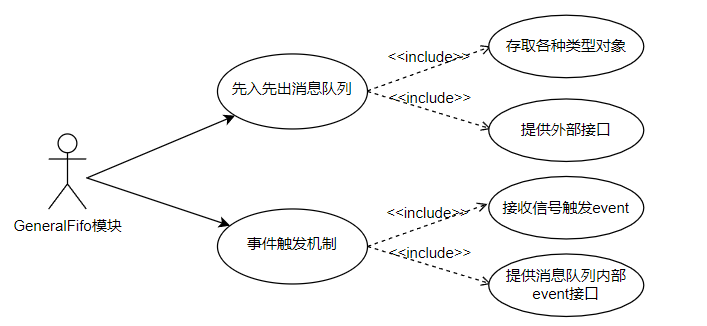
\includegraphics[width=0.75\textwidth]{GeneralFifo用例图.png}
    \caption{GeneralFifo模块用例图}
    \label{fig:badge}
\end{figure}

图3.1列举了GeneralFifo模块的功能需求。GeneralFifo作为一个先入先出队列需要满足
先入先出队列的所有功能,能够存储各种类型的对象,提供队列内部的一些基础接口如:
队列深度、存对象方法以及取对象方法等等。其次,GeneralFifo为了满足仿真平台能够
实现各个模块之间即时的消息传递,GeneralFifo需要实现当队列接收到消息时,便触发
相应的事件的功能,并且GeneralFifo模块需要提供模块内部的事件相关接口,以便其他模块
可以接受到队列内部的事件触发。

\subsection{Processor模块功能需求}
Process模块包括DSP、HAC以及DMA三种不同的硬件模型,Processor模块需要实现各个硬件
模型各自的功能需求以及硬件模块与其他模块之间的交互功能。Processor模块的用例图如
下图3.2所示:

\begin{figure}[h]
    \centering
    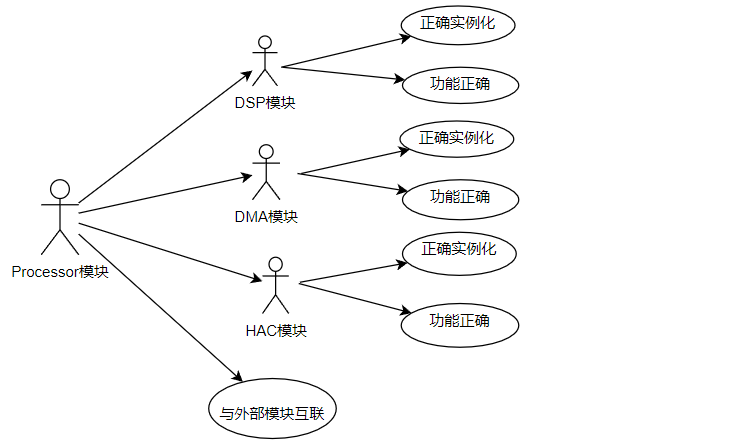
\includegraphics[width=0.75\textwidth]{Processor模块用例图.png}
    \caption{Processor模块用例图}
    \label{fig:badge}
\end{figure}

图3.2列举了Processor模块的整体需求,包括DSP、HAC和DMA三种硬件模型的功能需求以及
所有硬件模型与其他模块的交互功能需求,包含与Memory模块和调度器模块的交互。下面就
这几个方面分别来详细介绍Processor模块的功能需求。

DSP模块需要实现在仿真平台构建时,根据硬件平台配置文件中的信息正确实例化,保证
具体DSP实例能够通过总线连接到整个仿真平台中且DSP实例的配置信息正确。同时DSP模块
在实例化后需要实现自己的硬件功能:接收并处理来自DMA实例或者调度器模块
的任务实例,并根据任务实例中提取出的信息正确执行任务,并发送消息到下一级硬件实例
中。

HAC模块与其他Peocessor模块的一样需要在仿真平台构建时能够正确实例化。同时HAC模块
在实例化后需要实现自己的硬件功能,HAC模块作为一个用于处理某一种特定的任务的硬件
模块,其需要接收并处理来自调度器的任务实例。接收需要根据任务信息从特定地址的内存
块取出数据,然后以一定的时延处理任务,并在任务处理结束后将数据存储到特定地址的内
存中。在这个过程中需要保证任务处理时延正确、搬入搬出的数据正确。

DMA模块同样需要在仿真平台实例化的时候能够正确实例化。与此同时,DMA模块需要完成
其模块的功能,即与Memory模块进行交互,进行数据的搬入搬出,保证在数据的搬入搬出的
过程中数据的正确。并且DMA模块能够和其他模块进行消息交互,与DSP模块之间形成任务的
执行流水线。

Processor模块需要能与其他模块进行消息以及数据的交互,需要保证消息传递的及时性
以及正确性,保证数据传输时源地址和目的地址的正确以及数据本身的正确。

\subsection{Memory模块功能需求}
Memory模块需要实现能够成功实例化且模块功能正确,以及需要保证能够和其他模块进行
消息交互以及数据传输的功能。Memory模块的用例图如下图3.3所示:

\begin{figure}[h]
    \centering
    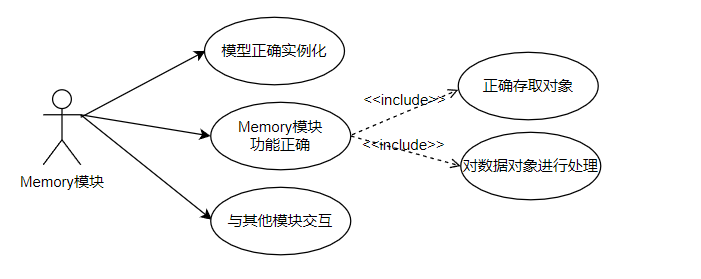
\includegraphics[width=0.75\textwidth]{Memory模块用例图.png}
    \caption{Memory模块用例图}
    \label{fig:badge}
\end{figure}

如图3.3所示,Memory模块需要实现模型能够正确实例化、Memory模块基础功能以及外部模块
之间消息交互的功能。这几部分需求的具体内容如下:

1、Memory模块能够在硬件平台搭建时根据硬件平台配置文件的信息去实例化,并通过
模块上实例化的Port与总线连接,从而与整个硬件平台连接在一起。

2、Memory模块需要保证其在实例化后,Memory实例的功能正确:Memory模块能够接收来自其他模块的
存取对象的请求,并根据请求的类型以及具体任务信息执行任务,在执行数据的存取时保证数据以及存取
地址的正确性。

3、Memory模块在执行数据存取的时候需要通过总线与其他内存模块进行数据的交互、通过GeneralFifo
消息队列与调度器模块中的内存管理模块、DMA实例以及HAC实例进行消息的交互,通知数据存取任务的
开始以及结束。

在介绍完仿真平台中硬件平台的功能需求之后,本文从仿真平台的使用用户的角度来介绍仿真平台的功
能性需求。如表3.2所示,仿真平台使用所涉及到的需求用户分为普通用户1、高级用户和普通用户2三类。
下面将对这三种用户的需求进行详细的分析。

\subsection{普通用户1需求}
普通用户1即是简单使用仿真平台进行业务仿真的用户。普通用户1的用例图如下
图3.4所示:

\begin{figure}[h]
    \centering
    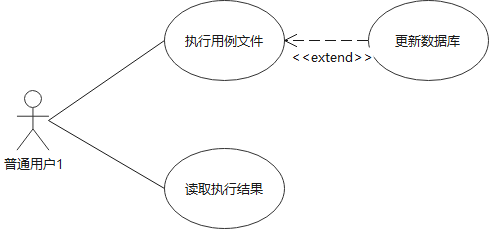
\includegraphics[width=0.75\textwidth]{普通用户1用例图.png}
    \caption{普通用户1用例图}
    \label{fig:badge}
\end{figure}

图3.4列举了普通用户1对仿真平台的执行用例文件功能、读取执行结果功能以及
仿真结果及仿真执行信息数据存储的需求,接下来对每个功能的具体需求进行阐述。
普通用户1的执行用例文件用例图如图3.5所示:

\begin{figure}[h]
    \centering
    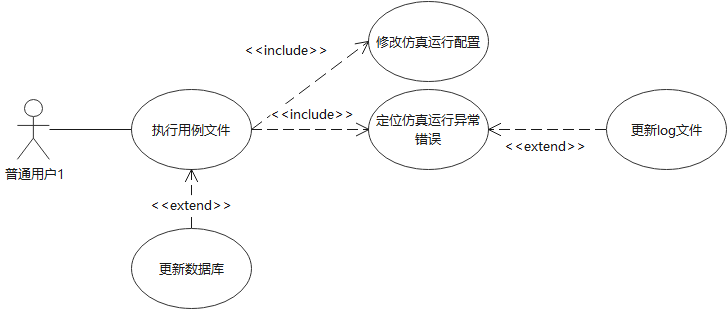
\includegraphics[width=1\textwidth]{普通用户1执行用例文件用例图.png}
    \caption{普通用户1执行用例文件用例图}
    \label{fig:badge}
\end{figure}

如图3.5执行用例文件用例图所示。执行用例文件功能分为修改仿真运行配置、
定位仿真运行异常错误和查看用例执行结果信息几个子功能。执行用例文件功
能及其子功能的需求具体内容如下:

1、	仿真结果时序正确。仿真时序正确要求每个任务的执行时间以及整体任务的
执行调度顺序与输入的任务用例文件中任务信息以及任务间的依赖关系一致。仿真
执行的输入是用例Excel文件,用例文件是将真实的任务在单板上的执行流程、执行
信息以及执行结果体现在文件中,通过解析文件信息,将任务真实的具体信息及依赖
关系作为仿真输入,通过任务调度平台的正确调度使得整个仿真最终得以正确执行。

2、	仿真运行可配置。因为仿真平台需要的执行用例主要用于基带芯片上,所以用例可
能存在多小区多信道的用例同时执行或者不同的用例同时混合执行,所以我们需要
在仿真运行前配置用例执行次数、仿真执行的用例文件名称、硬件配置文件名称以
及log文件和数据库文件的位置,这样就能适配不同情况下的仿真。用户可以仅仅
、修改执行脚本中的数据即可对整个仿真执行过程进行修改,从而得出用户所需的
不同的仿真结果。

3、	定位仿真执行异常错误。任务用例在仿真过程中可能会遇到各种情况的错
误,有些是用例文件的任务信息错误,有些是任务执行时的错误。我们需要能
够迅速定位到错误位置,我们通过任务执行过程中细致的log记录,可以迅速
定位到任务执行哪一级出现错误以及可以查询到各个模块之间数据传输在总线
上哪一级出现问题,可以迅速地定位到问题的产生地方以及解决问题。

以上详细的介绍了普通用户1对仿真平台执行仿真用例的具体需求,包括在仿真过程
中通过数据库将详细的任务执行信息记录下来。

用户执行用例仿真的最终需求还是为了得到用例仿真结果信息。我们在仿真过
程中通过数据库记录硬件平台的具体信息(如核一段时间的利用率、内存碎片
等等)和任务执行的具体细节(任务的提交时间、开始时间、结束时间等等)。
用户可以通过访问数据库文件来查看用例执行结果信息,从而得出自己所需要的
的信息。数据库文件需要记录多次的仿真结果,不同的仿真结果以SimId为标志区
分,并记录仿真执行的平台、仿真的时钟频率、执行的用例文件等等该次仿真的具
体信息。这样我们可以将我们需要的执行的多次用例通过脚本依次执行,最后也可以
查看到每次仿真执行后的具体信息。

\subsection{高级用户需求}
高级用户即是那些深度使用和开发该仿真平台的用户,除了普通用户1的需求,
他们还需要对仿真平台的配置修改需求。高级用户的用例图如下图3.6所示:

\begin{figure}[h]
    \centering
    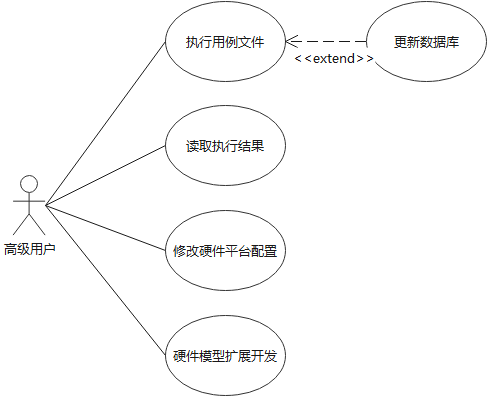
\includegraphics[width=0.7\textwidth]{高级用户用例图.png}
    \caption{高级用户用例图}
    \label{fig:badge}
\end{figure}

图3.6列举了高级用户仿真运行、读取仿真运行结果信息、修改硬件平台配置
和硬件模型扩展开发的需求。接下来我们对高级用户比普通用户1多出的两种
功能需求进行详细的阐述。

因为在芯片设计过程中,高级用户需要尝试手动修改仿真平台中硬件平台中不
同的硬件配置去运行仿真,因此我们的硬件配置需要高级用户能够很方便能够
去修改。仿真平台中硬件平台的构建是通过解析输入的硬件配置文件来进行的,
仿真平台输入的硬件配置文件类型包括Excel表及XML文件,用户可以通过
修改硬件配置文件中的硬件配置信息来达到他们对硬件配置进行修改的需求。

高级用户包括仿真平台的开发人员,芯片上的硬件不是统一不变,不同的硬件
行为不同,因此当出现不同的硬件时,开发人员需要对新的硬件进行建模。但现有
芯片中的硬件类型大致就几种类型,该仿真平台基于硬件类型对各种硬件进行区分,为了
赢家女建模操作更加方便,仿真平台统一构建了各种类型硬件的基类,建模时用户只需基于
这几种基类进行扩展开发即可。这样高级用户就可以很方便的仿真平台进行二次开发。

\subsection{普通用户2需求}
普通用户2即是那些使用设计空间探索流程的开发人员,只关注设计空间探
索流程的输入输出以及一些参数设置。普通用户2的用例图如下图3.7所示:

\begin{figure}[h]
    \centering
    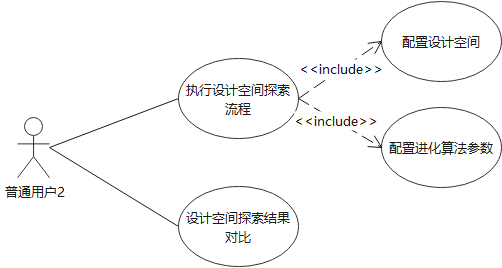
\includegraphics[width=0.7\textwidth]{普通用户2用例图.png}
    \caption{普通用户2用例图}
    \label{fig:badge}
\end{figure}

由图3.7可见,普通用户2关注设计空间探索流程的输入输出以及流程中一些
参数设置,对设计空间探索流程中具体执行过程并不关心。设计空间探索流
程的输入是目标值及其组成的设计空间和仿真模型。在流程中可以调整一些
进化算法的参数,如进化算法代数以及交叉变异的概率等等。我们通过在设
计空间探索流程执行脚本中设置相应的参数,就可以方便的调整设计空间探
索流程中遗传算法模块相应的参数,去得到对应的结果。最后能输出一
个种群的帕累托最优解集。

普通用户2可以通过设置的结果分析脚本使最后输出的脚本与原设计参数下执行结果进行对比,更加方
便可视化的得出用户所需要的结论。以便用户得出所需的设计参数或者进行下一轮的设计空间探索流程,
接下来对系统的非功能需求进行阐述。

\section{非功能需求}
仿真平台及设计空间流程整个系统在满足功能需求的基础上,还要根据系统的
实际情况,满足非功能需求。对于整个系统而言,非功能需求主要体现在可扩
展性、可维护性和性能需求上。这些非功能需求的作用对项目来说也是至关重
要的,只有同时满足功能性需求和非功能性需求,该应用才能在项目中顺利地
发挥其作用。

\subsection{可扩展性需求}
系统主体的仿真平台整体逻辑比较复杂,涉及5大模块,在各个模块内部有很多
部分功能类似,代码复杂,有很多模块需要复用。同时由于硬件设计的变化,
我们需要对硬件模块在后续开发中要不断进行扩展,整个项目的可扩展性要求
高,所以为了实现可扩展性需求,我们将各大模块代码模块化处理,在外部设
计接口,统一通过接口进行交互。模块内部功能相似的模块统一设计基类,通
过继承基类进行扩展开发。减少代码之间的循环依赖和降低代码之间的耦合,
从而提高系统的开发效率以及后续的扩展功能,使得系统满足可扩展性需求。

\subsection{可维护性需求}
在仿真建模以及仿真平台的搭建过程中,系统功能的实现并不能一劳永逸,在
新的硬件模块的增加后,仿真平台的功能以及性能是否满足要求,需要后续的
不断对其进行维护,才能保证仿真平台的稳定性和可用性。为了实现仿真平台
的可维护性,我们通过将仿真平台功能组件化,以保证后续模型的添加在功能
实现方面可以实现复用,更好的兼容现在的平台。降低了模型的开发难度以及
方便了后续开发人员对功能和组件的维护,提高了开发效率。

同时,因为仿真平台的输入也一直在变,我们设置了一个迭代平台,可以每天
在服务器上进行不同用例的自动化仿真,并给出仿真结果,降低了开发人员的
人工成本。

\subsection{仿真平台轻量级需求}
该仿真平台是建立在实现设计空间探索流程的需求之上。由于设计空间的庞大,
即使在对设计空间进行剪枝之后在设计空间探索流程中所要进行的仿真次数依
旧很多,原有基于SystemC的仿真验证平台就不再适用于当前的场景下了,因此
基于Simpy的仿真引擎我们重构了现有的仿真平台。对于仿真平台的轻量级需求
是指仿真平台构建迅速,单次仿真执行时间短以及在每次仿真结束能够快速提取
出所需要的目标参数。

\subsection{性能需求}
仿真平台主要是为了进行业务行为仿真,设计空间探索的目的是为了得到在各个方面
结果都表现优秀的设计方案解集。所以评价仿真平台性能的指标包括仿真结果的时序
准确以及仿真执行的速度,评价设计空间探索流程的性能是观察其输出结果是
否在各个方面都体现了优秀的性能以及设计空间探索流程的效率。在这里我们
也将这些作为性能需求的评价指标。

首先,在仿真平台方面,我们将输入的用例文件解析为以任务和数据为节点的
有向无环图,这保证了任务执行的顺序,任务执行时间的准确则体现了硬件模
型行为的准确。为了仿真能够更快的执行,我们简化了硬件模型的行为,以软
件行为替代硬件行为,在内存模型上我们简化了数据的格式,将真实的数据存
取过程只是体现在仿真时延的增加,而不是真实的进行存取。且采用了SimPy
仿真框架,从而实现仿真速度的提升。

其次,在设计空间探索方面,我们采用进化算法,并通过进化算法的选择和具体
的算法设置保证结果是全局最优而不会陷入局部最优。我们同时也需要保证设计
空间探索流程的速度,保证整个设计空间探索流程能在很短时间闭环,以方便设
计人员能在设计空间探索流程结束后很快的对设计探索的结果进行分析,得出所
需要的设计架构。由于我们采用进化算法,我们在每一代中,对于相应的参数,
我们都要通过仿真得到对应的仿真结果并且提取出我们需要的结果。因此我们通
过在设计空间探索过程中将仿真模型通过机器学习简化为仿真预测模型,这样能
大大减少每一次的对对应设计参数得出结果的时间,从而达到极大的提高设计空
间探索流程的效率的需求。性能需求表如下表3.3所示:

\begin{table}[htb]
    \centering\normalsize
    \caption{性能需求表}
    \begin{tabular}{|c|c|c|ll}
    \hline
    模块       & 需求项           & 需求值               \\ \hline
    仿真平台构建模块 & 仿真硬件平台搭建成功的时间 & \textless{}=5s    \\ \hline
    仿真执行模块   & 单次单小区仿真执行的时间  & \textless{}=150s   \\ \hline
    仿真执行模块   & 仿真结果时序与用例一致   & true              \\ \hline
    设计空间探索模块 & 设计空间探索结果全局最优  & true              \\ \hline
    \end{tabular}
    \end{table}

\section{本章小结}
本章从实际场景出发,根据业务仿真的真实场景和设计空间探索流程的真实场景
,详细分析了整个系统的功能需求和非功能需求,在对产品的需求进行了简介之
后,给出了用户需求列表。在功能需求中,根据不同用户对系统的需求,对功能
需求进行了详细的阐述,描述了用例文件执行、查看仿真结果信息、执行设计空
间探索流程和得到设计空间探索结果对比等功能需求。接着根据系统的实际情况,
从可扩展性、可维护性和性能需求几个方面来详细阐述系统的非功能需求。
这一章对仿真平台及设计空间探索流程的需求进行了比较明确地阐述,为后续的
系统概要设计打下了基础。
% !TeX root = ../main.tex

\chapter{概要设计}
本章是在需求分析的基础上对整个仿真平台我所完成的模块设计及设计空间探索
模块的设计进行简要的阐述。在此章节中,我们可以清晰的了解到硬件模型生成模块
(Processor模块和Memory模块)、GeneralFifo模块设计及设计空间探索的流程,
为具体实现打好基础。

\section{系统整体结构}
整个系统整体结构主要包括两个部分:仿真平台部分,包括硬件平台
构建、调度器模块、任务图解析及仿真部分;设计空间探索部分,包
括通过脚本迭代生成训练集、训练预测模型及运用遗传算法实现设计
空间探索。系统的整体架构图如图4.1所示:

\begin{figure}[h]
    \centering
    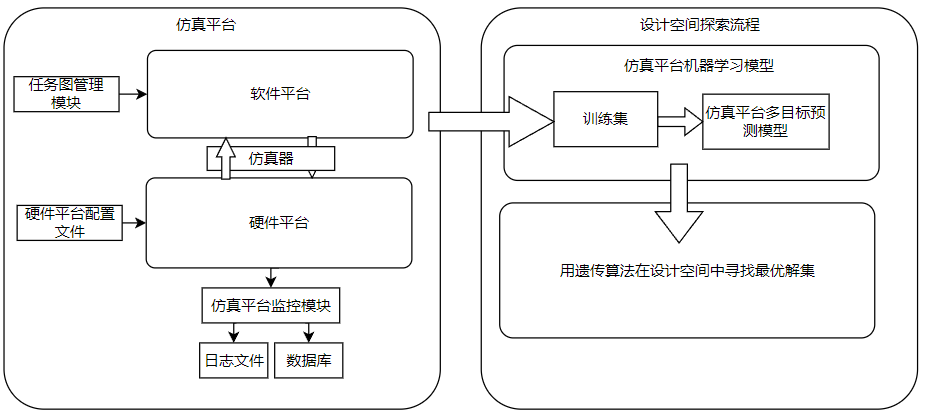
\includegraphics[width=1\textwidth]{系统整体框架图.png}
    \caption{系统整体框架图}
    \label{fig:badge}
\end{figure}

如系统整体框架图可以看出,该系统是一个以仿真平台为基础,实现
通过遗传算法对比较大的设计空间进行探索。我们初期实现TopLevel
仿真平台,仿真平台通过读取硬件配置表实例化硬件平台。随后平台
读取输入的任务图,软件平台读取任务,然后通过调度分到各个硬件
上执行任务,输出日志文件和数据库文件。

通过在仿真平台上快速进行仿真,得出相对于设计空间较小的训练集
文件。训练集文件中包括硬件平台配置,如总线位宽、一个组中DSP
数量、内存大小等等。还包括仿真输出的数据库中提取的仿真信息
,如仿真时延、核利用率、核一致性等等。

然后基于生成的训练集文件,通过现有的机器学习Adaboost模型\cite{29}对
训练集文件训练出仿真平台多目标预测模型\cite{30},最后我们运用遗传算
法对设计空间进行迭代剪枝,最后得出最优的设计种群。

系统主要包括仿真平台和设计空间探索流程两个部分,所以下面就
这两个方面以及仿真结果数据库部分来分别来简要介绍各自的设计。

\section{仿真平台硬件模型生成模块概要设计}
TopLevel仿真平台主要实现硬件平台各个模块的实例化,任务图的
读取以及执行。整个仿真平台模块主要分为ALA调度器模块、Memory
模块、总线模块、处理器模块、用于各模块之间数据以及消息传输的
GeneralFifo模块。仿真平台的整体架构图如图4.2所示:

\begin{figure}[h]
    \centering
    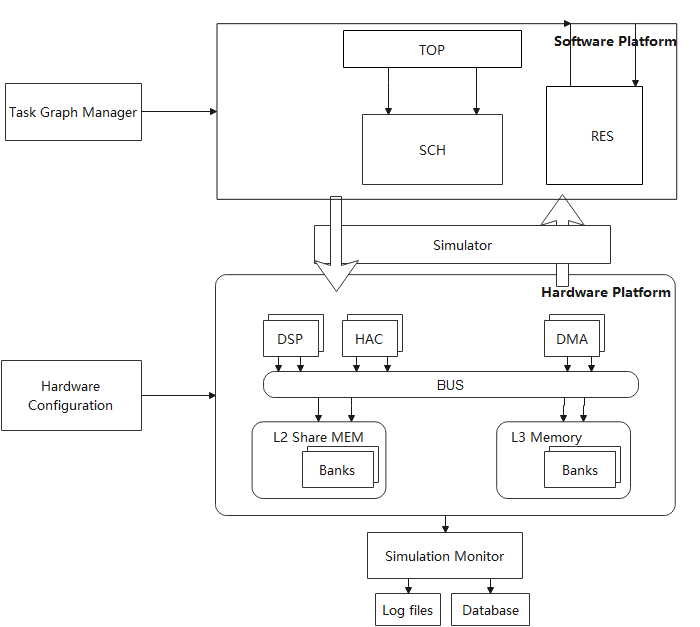
\includegraphics[width=1\textwidth]{仿真平台整体架构图.png}
    \caption{仿真平台整体架构图}
    \label{fig:badge}
\end{figure}

下文主要对仿真平台中设计实现的的硬件平台构建模块、硬件模型生成模块
(Processor模块和Memory模块)以及GeneralFifo模块设计进行简要的介绍。

\subsection{硬件平台构建模块概要设计}
平台开发人员根据仿真平台用户的需求进行建模,提供在系统仿真过程中所需要的各种硬件
模型,用户根据需求构建系统仿真所需的硬件平台。在构建硬件平台时,用户通过修改硬件
平台配置文件中的硬件模块实例信息以及各个实例之间的连接方式,包括每个硬件模块的配
置信息和总线的路由映射。硬件平台的构建过程由下图4.3所示:

\begin{figure}[h]
    \centering
    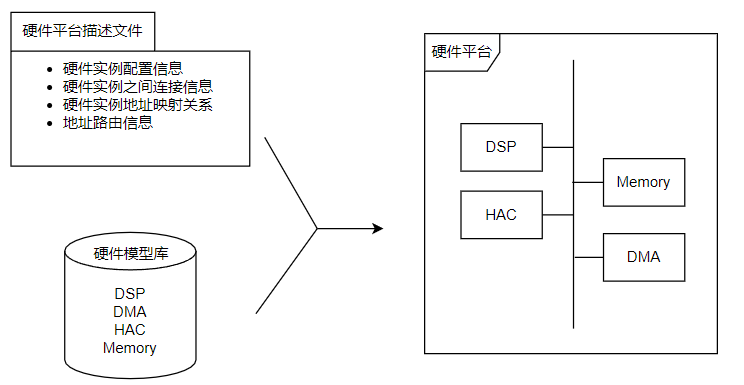
\includegraphics[width=0.8\textwidth]{硬件平台生成图.png}
    \caption{硬件平台生成图}
    \label{fig:badge}
\end{figure}

在仿真平台中,整个硬件系统的构成是一个树状结构的层次化架构,在硬件平台的构建
过程是对该树状结构进行深度优先遍历,所有硬件模型都基于GeneralModule基类实例化。
在硬件平台构建过程中会根据硬件平台配置文件中的配置信息,先实例化最下端叶节点的
各个具体的硬件模型,再去构建上层的分区组件直至整个硬件平台实例化完成。硬件平台
构建的活动图如图4.4所示:

\begin{figure}[h]
    \centering
    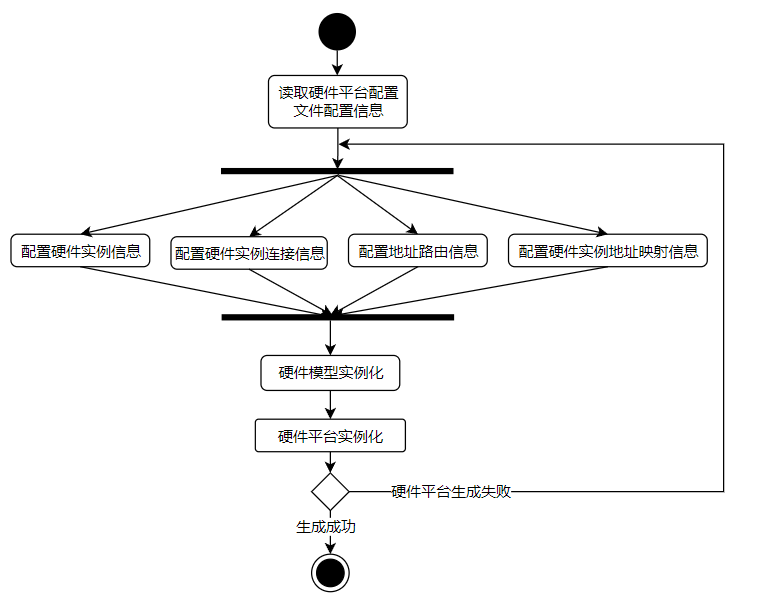
\includegraphics[width=0.9\textwidth]{硬件平台生成活动图.png}
    \caption{硬件平台生成活动图}
    \label{fig:badge}
\end{figure}

如图4.4所示硬件平台在构建过程中,平台需要从硬件模型库中实例化具体的硬件模型
。平台开发人员需要对各种硬件模型进行建模,包括DSP模型、DMA模型以及Memory模型
等等。在构建过程中,系统通过硬件平台配置文件中的硬件模型配置信息去修改硬件模型
库中的硬件模型基类中的可配置参数去实例化具体的仿真平台所需要的硬件模型。在将
建模好的硬件模型基类增加到硬件模型库中之前,通过对硬件模型的单点测试去修改和完善
在设计阶段没有考虑完善的功能需求。同时由于在不同的业务背景下,仿真平台需要不同的硬件
模型,但整体模型基础功能大致相同,所以我们在后续开发其他硬件模型时,只需基于现有
的硬件模型基类去开发,而不需要从零再进行开发。硬件模型库中涉及到多种硬件模型,其中
包括处理器硬件模型、调度器模型、存储器模型以及互联互通模型等。其中处理器模型、存储器
模型的概要设计将在后续几个小节中介绍。

\subsection{GeneralFifo模块概要设计}
GeneralFifo是为了满足模型处理流程需求而开发的一种通用先入先出队列(First in first out,Fifo)
机制\cite{31},可以实现/建模过程中各种前后级同步,反压等需求。它主要有以下几个方面的功能:

\begin{enumerate}
    \item 对连续的数据流进行缓存,防止在存储操作的时候发生数据丢失;
    \item 数据集中起来进行进栈和存储,可避免频繁的总线操作,减轻CPU的负担;
    \item 允许系统进行DMA操作,提高数据的传输速度。
    \item 作为消息队列,支撑仿真平台各个模块之间消息交互,提供事件触发机制。
\end{enumerate}

在硬件设计中,Fifo一般设计为“乒乓”存储方式,在硬件仿真设计中,我们采用以先入先出队列为
存储数据的存储器,GeneralFifo还集成了SimPy里的event机制,实现仿真平台中模块与模块之间的消息交互需求。

GeneralFifo模块通过在模块实例化的时候创建向空队列写对象事件以及从满队列中取
对象事件,当相对应操作出现时,便通过SimPy中的event机制去触发相对应的事件。而
等待该操作的外部模块就可以即时接收到讯息,并即刻执行相对应的操作。这样就实现了
各个模块之间通过GeneralFifo通讯时,当没有对象,进程可以一直等待其他模块传对
象的情形。与此同时,为了实现整个GeneralFifo的事件触发机制,GeneralFifo需要提供队列是
否为空或为满、获取队列的深度以及队列中对象的数量、获取向空
队列写对象事件和从满队列中取对象事件等方法和函数接口。GeneralFifo模块实现流程如图4.5所示:
\\
\\
\\

\begin{figure}[h]
    \centering
    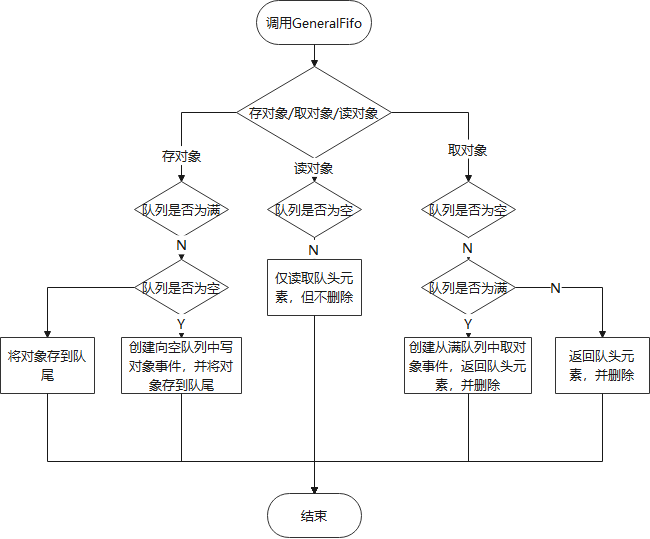
\includegraphics[width=1\textwidth]{GeneralFIFO流程图.png}
    \caption{GeneralFifo流程图}
    \label{fig:badge}
\end{figure}

\subsection{Memory模块概要设计}
Memory模块\cite{32}在整个硬件平台中包括SL2(外部的公共内存池)和PL2
(在每个processor模块内部的内存池)两种内存块。Memory模块根据平台配置
的Bank位宽在模型内部将Memory分为不同的Bank模块,具体的数据读写由内部
Bank模块进行执行。

Processor模块对数据的处理需要从SL2内存池中将数据取到自己内部的PL2内存池中,
再将处理后的数据存到外部的SL2内存池中。Memory模块负责数据的存取处理。Memory
模块接收从总线上传来的读写请求Flit,并根据
位宽将Flit拆分为相应的Bank操作,并将操作处理符发送到到对应Bank
上的Fifo中。Bank模块在硬件平台构建时进行初始化,同时Bank模块创
建bank读写操作进程,一旦有bank读写操作符发送到对应的Fifo中时,
就会触发从Fifo中取出bank读写操作对象,完成开辟bank读写操作符上
所带的读写操作信息,开辟对应地址的内存空间并存储数据或将对应地址
的数据取出并释放该地址的内存空间,并向Memory上的SlavePort
发送读写响应。Memory模块的结构图如图4.6所示:
\\

\begin{figure}[h]
    \centering
    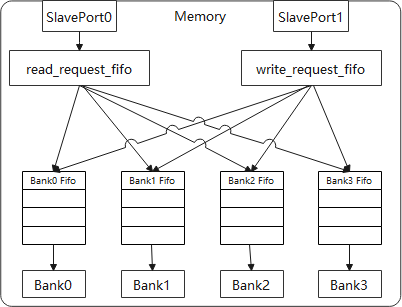
\includegraphics[width=0.8\textwidth]{Memory模块结构图.png}
    \caption{Memory模块结构图}
    \label{fig:badge}
\end{figure}

读写请求通过总线发送到对应Memory模块的SlavePort口,根据请求类型不同
分别发到读请求Fifo上或写请求Fifo上,再根据Bank位宽拆分,发送
到不同Bank上的Fifo中排队,最后由相对应的Bank进行读写请求操作。

\subsection{Processor模块概要设计}
Processor模块对DSP、HAC和DMA三种模型进行建模,实现模型的硬件行为、
建立模型内的流水线结构并实现与其他模块的交互行为\cite{33}。Processor模块现在包括
ProcessorMgnt、ProcessorBase以及具体的DMA、DSP、HAC模型
模块。Processor模块整体结构如图4.7所示:
\begin{figure}[htb]
    \centering
    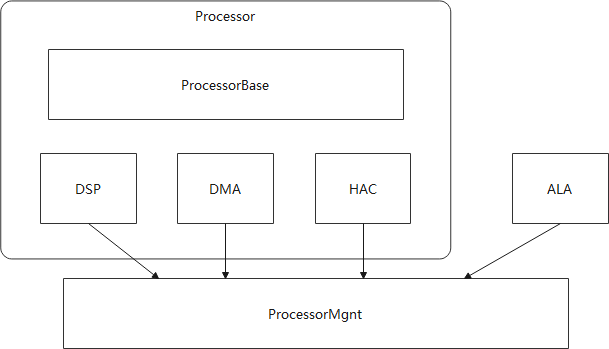
\includegraphics[width=0.8\textwidth]{Processor模块结构图.png}
    \caption{Processor模块结构图}
    \label{fig:badge}
\end{figure}

ProcessorMgnt模块是实现具体模型的管理功能。各个模型(ALA、DSP、
DMA等等)在实例化的时候,ProcessorMgnt记录下对应的对象,并提供
方法给各个模块之间通过内部的Fifo之间交互。这样我们在具体模块之间
进行消息交互的时候不用将消息封装成数据通过总线交互,节省了仿真时
的资源浪费。由于各个模块之间消息交互十分频繁,所以这样也大大提高
仿真平台的仿真效率。

ProcessorBase模块是DMA、DSP及HAC模块的基类,实现了具体模型的基
础功能,并提供相应的接口。ProcessorBase模块实现了模块消息交互以及
添加消息交互接口的功能。

DMA(direct Memory Access, 直接存储器访问)模块负责将数据从一块地
址复制到另一块地址空间,提供在存储器和存储器之间的高速数据传输,在
设计的仿真平台中主要负责PL2内存池和SL2内存池之间的数据传输。

DSP(Digital Signal Processing,数字信号处理)芯片是一种快速强大的微处理器,可以迅速的实现各种数字信号处理算法。
在仿真过程中,DSP模块负责快速完成数据的计算处理。在轻量级仿真平台中,该模块只有数据处理的
时延,不负责数据搬运。只需要体现系统时延,不需要对搬运的数据进行真实的操作。

HAC(Hardware Accelerator,硬件加速器)是用来专门处理某一类执行次数很多的硬件操作的
的硬件,为了加快这一类的操作,特地设计一种芯片专门处理这种操作。HAC模型负责处理
数据搬入、数据处理以及数据搬出的所有操作。

DMA(direct Memory Access, 直接存储器访问)模块负责将数据从一块地
址复制到另一块地址空间,提供在存储器和存储器之间的高速数据传输,在
设计的仿真平台中主要负责PL2内存池和SL2内存池之间的数据传输。

DSP芯片是一种快速强大的微处理器,可以迅速的实现各种数字信号处理算法。
在仿真过程中,DSP模块负责快速完成数据的计算处理,在该模块只有数据处理的
时延,不负责数据搬运。在DSP模块只需要体现系统时延即可。

\section{设计空间构建模块及仿真预测模型概要设计}
设计空间探索是指根据系统设计所关心的参数而对不需要的参数进行系统
分析和修剪。设计空间探索模块实现在可配置的系统资源构成的设计空间中
寻找目标优秀的设计方案。设计空间探索主要分为构建设计空间和选择优化目标、对
设计空间进行剪枝以及对设计空间探索结果分析三个部分。设计空间构成
由可配置的系统参数以及系统参数的可行范围构成,一般而言,设计空间
的整体范围会比较大。优化目标则是我们对整个系统的优化方向,比如在
本文中的设计空间探索流程中,优化目标为仿真时延、核利用率以及核一
致性几个参数。设计空间探索的流程图如图4.8所示:

\begin{figure}[htb]
    \centering
    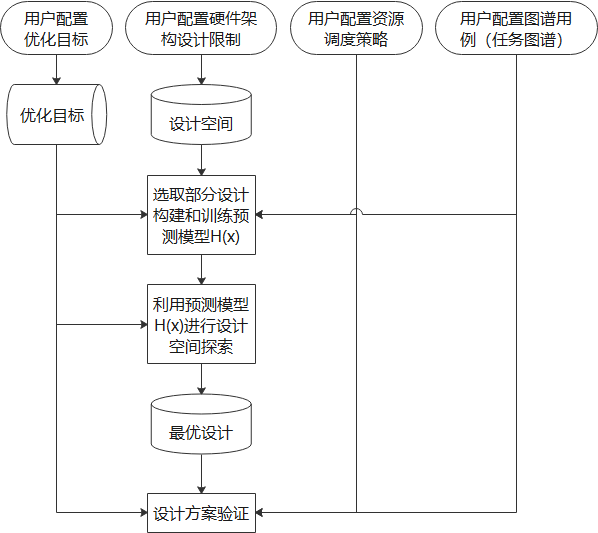
\includegraphics[width=0.9\textwidth]{设计空间探索流程图.png}
    \caption{设计空间探索流程图}
    \label{fig:badge}
\end{figure}

我在设计空间探索模块主要负责的是设计空间的参数提取和构建以及仿真
平台预测模型的设计与实现。

仿真系统中设计空间探索设计流程如图所示,在设计探索流程的具体实现中,
我们先修改仿真平台系统参数,自动化迭
代运行仿真平台,并通过读取数据库信息提取出设计空间探索所有的目标
值,最后将设计方案和对应的仿真数据输出到txt文件中。

将上个流程中提取的6000个训练集数据作为输入数据训练仿真平台预测模
型。最后在遗传算法中探索设计空间中所有设计方案,最后输出最为优秀
的设计种群作为我们设计的备选方案,并对方案重新在仿真平台上运行,
对仿真结果进行对比分析。

下面主要分别设计空间构建模块、探索预测模块的概要设计
进行简要介绍。

\subsection{设计空间构建模块概要设计}
通过对系统设计空间探索的需求分析,找出我们所需要的系统的优化方
向即优化目标,通过分析仿真系统哪几个可配置参数会对优化目标产生较
大影响,提取出这几个设计参数,根据真实芯片设计的参数变化,对设计
参数范围进行限制,最后形成设计空间。
通过对系统设计空间探索的需求分析,我们找出我们需要对系统的优化方
向即优化目标,通过分析仿真系统哪几个可配置参数会对优化目标产生较
大影响,提取出几个设计参数,通过对设计参数范围的限制,最后形成设
计空间。

由于后期在遗传算法进行设计空间探索的过程中进行迭代时,设计空间中
配置参数值的变化要求仿真平台中进行配置参数的调整。

\subsection{仿真平台预测模型概要设计}
设计空间探索流程中遗传算法需要进行多次的仿真过程迭代,为了减少设计
空间探索流程的时间开销,由于在设计空间探索的过程中,仿真平台的配置
参数和目标值固定,所以将系统仿真流程设计成仿真平台预测模型,这样可以大
大减少目标值的输出时间。接下来从训练集生成和预测模型生成两个方面介绍:

训练集生成模块实现的功能包括:读取设计空间中配置并配置到硬件配置
文件中、自动化读取配置文件迭  代运行仿真文件、读取每次仿真结果数据
库文件提取所需要的目标值、将设计方案和对应的目标值输出到文件中并
最终输出训练集文件。该模块的流程图如图4.9所示:

\begin{figure}[htb]
    \centering
    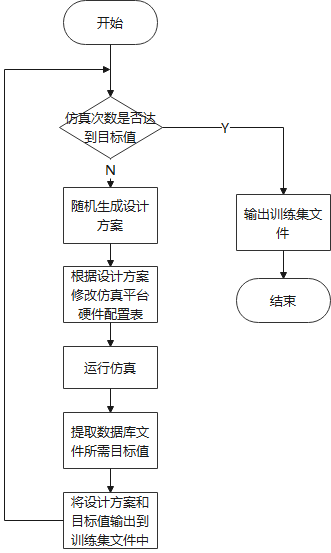
\includegraphics[width=0.5\textwidth]{训练集生成模块流程图.png}
    \caption{训练集生成模块流程图}
    \label{fig:badge}
\end{figure}

训练集文件中的目标值即仿真数据结果,我们需要在每次通过修改硬件配置
在仿真平台上进行系统仿真,在仿真结束后通过对数据库文件中数据的提取
将相应的目标值统计计算到相应的文件中。这样从设计空间中采样得到样本
,将样本在仿真平台上运行得出相应的目标值,从而得到训练集文件。

预测模型生成模块生成仿真平台多目标预测模型,先将上个流程中的数据集经过处理
后提取出来,并分为训练集和验证集。采用现有的sklearn框架中的决策
树回归模型\cite{34}去训练每个目标,再通过一个多目标预测模型类将所有模型
文件读取,并实现预测目标值的功能函数。这样整体每个目标的预测误
差较低。

\section{仿真信息数据库概要设计}
在仿真过程中,我们在每个节点对仿真信息进行统计,最后在仿真结束时
输出至数据库进行整理。从而得到一系列我们对整个仿真过程每个任务的
执行过程,每个硬件的利用率,内存的申请情况,通过这些信息,我们就
可以对整个仿真进行分析,并通过这些输出结果进行下一步DSE架构探索。

仿真系统的结果输出主要通过log信息和数据文件实现,log信息主要统计
任务执行的细节信息,方便寻找调优的关键节点。数据库文件统计任务的
执行过程,每个硬件的利用率,内存的利用等等。仿真平台的数据库采用
python的SQLite库实现。系统中只需在仿真流程中在数据库中各自独立更
新数据库中各个表的数据,每个表的数据表基本独立,SimId是所有数据
表的主键,用于区别多次仿真之间结果。数据库的物理模型由下列各表
所示:

\begin{table}[!h]
    \centering\normalsize
    \caption{SimRecord表}
    \begin{tabular}{|c|c|c|c|c|c|}
    \hline
    \textbf{序号} & \textbf{字段名} & \textbf{字段说明} & \textbf{类型} & \textbf{是否为空} & \textbf{说明} \\ \hline
    1           & SimId        & 仿真序号          & int         & N             &             \\ \hline
    2           & StartTime    & 仿真开始时间        & int         & N             &             \\ \hline
    3           & EndTime      & 仿真结束时时间       & int         & N             &             \\ \hline
    4           & SimTime      & 仿真持续时间        & int         & N             &             \\ \hline
    5           & TestCaseName & 仿真用例名字        & Text        & N             &             \\ \hline
    \multicolumn{2}{|c|}{补充说明} &               &             &               &             \\ \hline
    \end{tabular}
    \note{注:一个数据库可以记录多次仿真的结果,以SimId作为区别。}
    \end{table}

\begin{table}[!h]
    \centering\normalsize
    \caption{AlaKernelTaskTbl表}
    \begin{tabular}{|c|c|c|c|c|c|}
    \hline
    \textbf{序号} & \textbf{字段名} & \textbf{字段说明} & \textbf{类型} & \textbf{是否为空} & \textbf{说明} \\ \hline
    1           & SimId        & 仿真序号          & int         & N             &             \\ \hline
    2           & KernelId     & Kernel任务序号    & int         & N             &             \\ \hline
    3           & InstId       & 任务具体实例序号      & int         & N             &             \\ \hline
    4           & KernelType   & 任务类型          & int         & N             &             \\ \hline
    5           & ReadyTime    & 任务的就绪时间       & int         & N             &             \\ \hline
    6           & IssueTime    & 任务开始执行时间      & int         & N             &             \\ \hline
    7           & CompleteTime & 任务结束执行时间      & int         & N             &             \\ \hline
    8           & PreMoveEnd   & 任务前搬移结束时间     & int         & N             &             \\ \hline
    9           & PostMoveEnd  & 任务后搬移结束时间     & int         & N             &             \\ \hline
    \multicolumn{2}{|c|}{补充说明} &               &             &               &             \\ \hline
    \end{tabular}
    \note{注:AlaKernelTaskTbl表记录的是在Dsp核执行的任务,前搬移任务和后搬移任务分别用来搬运任务的输入数据和输出数据。}
    \end{table}

\begin{table}[!h]
    \centering\normalsize
    \caption{HacJobTable表}
    \begin{tabular}{|c|c|c|c|c|c|}
    \hline
    \textbf{序号} & \textbf{字段名} & \textbf{字段说明} & \textbf{类型} & \textbf{是否为空} & \textbf{说明} \\ \hline
    1           & SimId        & 仿真序号          & int         & N             &             \\ \hline
    2           & JobTypeId    & 任务的序号         & int         & N             &             \\ \hline
    3           & InstId       & 任务具体实例序号      & int         & N             &             \\ \hline
    4           & PipeLine     & 任务具体哪一级流水     & int         & N             &             \\ \hline
    5           & StartTime    & 任务开始执行时间      & int         & N             &             \\ \hline
    6           & EndTime      & 任务结束执行时间      & int         & N             &             \\ \hline
    \multicolumn{2}{|c|}{补充说明} &               &             &               &             \\ \hline
    \end{tabular}
    \note{注:该表记录了Hac任务所处的流水级别和Hac任务在该级流水的执行细节。}
    \end{table}

\begin{table}[!h]
    \centering\normalsize
    \caption{WFEJobTable表}
    \begin{tabular}{|c|c|c|c|c|c|}
    \hline
    \textbf{序号} & \textbf{字段名} & \textbf{字段说明} & \textbf{类型} & \textbf{是否为空} & \textbf{说明} \\ \hline
    1           & SimId        & 仿真序号          & int         & N             &             \\ \hline
    2           & JobTypeId    & 任务的序号         & int         & N             &             \\ \hline
    3           & InstId       & 任务具体实例序号      & int         & N             &             \\ \hline
    4           & StartTime    & 任务开始执行时间      & int         & N             &             \\ \hline
    5           & CompleteTime & 任务结束执行时间      & int         & N             &             \\ \hline
    \multicolumn{2}{|c|}{补充说明} &               &             &               &             \\ \hline
    \end{tabular}
    \note{WFE任务不在核上执行,只起任务的收齐作用,当所准备的任务全部做完后,立刻执行完毕。}
    \end{table}

\begin{table}[!h]
    \centering\normalsize
    \caption{Pl2UsageRecord表}
    \begin{tabular}{|c|c|c|c|c|c|}
    \hline
    \textbf{序号} & \textbf{字段名} & \textbf{字段说明} & \textbf{类型} & \textbf{是否为空} & \textbf{说明} \\ \hline
    1           & SimId        & 仿真序号          & int         & N             &             \\ \hline
    2           & TTI          & 仿真时间段         & int         & N             &             \\ \hline
    3           & SimTime      & 记录的时间点        & int         & N             &             \\ \hline
    4           & AlaId        & 调度器Id         & int         & N             &             \\ \hline
    5           & PoolId       & 内存池Id         & int         & N             &             \\ \hline
    6           & UsedSize     & 内存池已使用的大小     & int         & N             &             \\ \hline
    7           & AllocSize    & 内存池已分配的大小     & int         & N             &             \\ \hline
    \multicolumn{2}{|c|}{补充说明} &               &             &               &             \\ \hline
    \end{tabular}
    \note{注:该表记录了Pl2内存的在每个时间段的使用情况,以内存池为单位进行记录。}
    \end{table}

\begin{table}[!h]
    \centering\normalsize
    \caption{SimUsageTable表}
    \begin{tabular}{|c|c|c|c|c|c|}
    \hline
    \textbf{序号} & \textbf{字段名}  & \textbf{字段说明} & \textbf{类型} & \textbf{是否为空} & \textbf{说明} \\ \hline
    1           & SimId         & 仿真序号          & int         & N             &             \\ \hline
    2           & ProcessorName & 硬件名称          & text        & N             &             \\ \hline
    3           & TTI           & 仿真时间段         & int         & N             &             \\ \hline
    4           & SampleCount   & 时间片序号         & int         & N             &             \\ \hline
    5           & Usage         & 时间片内硬件利用率     & int         & N             &             \\ \hline
    \multicolumn{2}{|c|}{补充说明} &               &             &               &             \\ \hline
    \end{tabular}
    \note{注:该表记录了在仿真过程中每个时间片内硬件资源的利用率。}
    \end{table}

\begin{table}[!h]
    \centering\normalsize
    \caption{DBMUsageRecord表}
    \begin{tabular}{|c|c|c|c|c|c|}
    \hline
    \textbf{序号} & \textbf{字段名} & \textbf{字段说明} & \textbf{类型} & \textbf{是否为空} & \textbf{说明} \\ \hline
    1           & SimId        & 仿真序号          & int         & N             &             \\ \hline
    2           & TTI          & 仿真时间段         & int         & N             &             \\ \hline
    3           & SimTime      & 记录的时间点        & int         & N             &             \\ \hline
    4           & AlaId        & 调度器Id         & int         & N             &             \\ \hline
    5           & PoolId       & 内存池Id         & int         & N             &             \\ \hline
    6           & UsedSize     & 内存池已使用的大小     & int         & N             &             \\ \hline
    7           & AllocSize    & 内存池已分配的大小     & int         & N             &             \\ \hline
    \multicolumn{2}{|c|}{补充说明} &               &             &               &             \\ \hline
    \end{tabular}
    \note{注:该表记录了仿真过程中以DBM管理的Sl2内存每个时间段的分配情况,以内存池为单位记录。}
    \end{table}

~\\
\section{本章小结}
本章基于仿真平台的的整体设计及设计空间探索的整体框架入手,详细介绍
了仿真平台的整体流程以及相关模块的架构以及功能实现、设计空间探索模
块的主要流程以及各个流程模块里面的功能实现,如何生成训练集以及预测
模型的训练生成等等。

本章为系统的详细设计提供了明确的框架,表明了设计开发的重点和难点,
为后续系统的具体设计提供了有力的帮助。
% !TeX root = ../main.tex

\chapter{详细设计与实现}
本章节是基于第四章概要设计的基础上,给出整个系统中的详细设计与实现,
主要内容包括仿真平台硬件平台构建和硬件模型建模的实现以及整个平台的仿真运行流程细节、设
计空间探索过程过程中训练集和多目标预测模型的生成以及对设计空间探索结果分析这些部分
的具体实现。

\section{仿真平台模块硬件平台构建模块的设计与实现}
仿真平台是基于任务图的一个以SimPy引擎为仿真框架的仿真系统\cite{36}。
仿真平台的设计与实现是整个系统实现部分的重中之重,而对仿真系统各个模
块的建模则是这部分工作的核心。
整个仿真系统通过解析输入的硬件配置文件,实例化硬件模块,通过总线将各个硬件
模块连接起来,形成整个仿真平台的硬件平台部分。任务图管理模块通过解
析输入的任务图,并根据触发关系链式的调度任务,将任务分配到具体的硬
件模型上执行。下面将详细阐述仿真平台硬件平台构建模块的功能实现及结构。

整个仿真平台的硬件平台部分从结构上可以抽象为一个自顶而下的一个树状结构,
所有具体的硬件模型实例都被视为该树状结构的最底端的叶子节点,所有的叶子节点(硬件模型实例)
都是由上层的节点(不同的子组件)分区管理,依次逐层向上。树的根节点即为仿真平台的
硬件平台部分。仿真平台的硬件平台的树状结构示意图如图5.1所示:

\begin{figure}
    \centering
    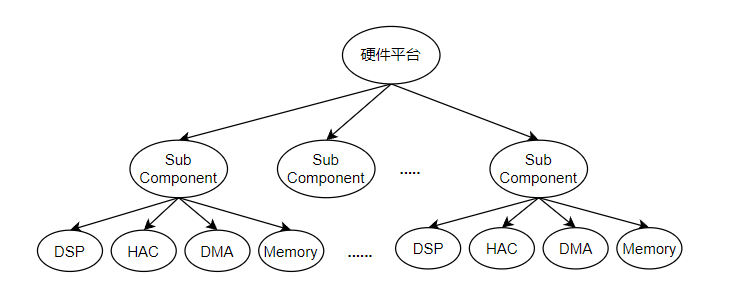
\includegraphics[width=1\textwidth]{硬件平台树状结构示意图.png}
    \caption{硬件平台树状结构示意图}
    \label{fig:badge}
\end{figure}

用户在进行仿真之前需要根据自己的需求去修改硬件平台配置文件,
硬件平台构建需要读取硬件平台配置文件并解析,系统所需的硬件平台配置文件包括
:V801.xml用来描述所有硬件模型之间的连接信息及Port信息、V801MemMap.xml
用来描述所有硬件模块模块与具体物理地址之间映射关系、V801MemPt.xml用来
描述内存模块的具体信息、V801Prop.xml用来描述所有需要实例化的模块包括
Processor和总线模块等等在实例化的时候的所需的所有具体信息、V801Route.xml
描述了所有实例化后的硬件模块之间的路由信息,将各个硬件模型通过总线连接形
成一个完整的硬件平台。在实际的用例仿真业务中,在进行用例仿真之前,仿真系统
先根据硬件平台配置文件对硬件平台进行构建。PlateformBuilder会实例化DSP、DMA
以及HAC等等硬件模型,当一个子组件中所有的硬件模块全部实例化后,再继续实例化
其他子组件中的硬件模块,最后当所有组件中硬件模块实例化成功后,整个仿真平台
的硬件平台就构建成功了。

我们通过创建SaeSimulator单实例去实现整个平台初始化的功能,整个SaeSimulator
的类图如图5.2所示:

\begin{figure}
    \centering
    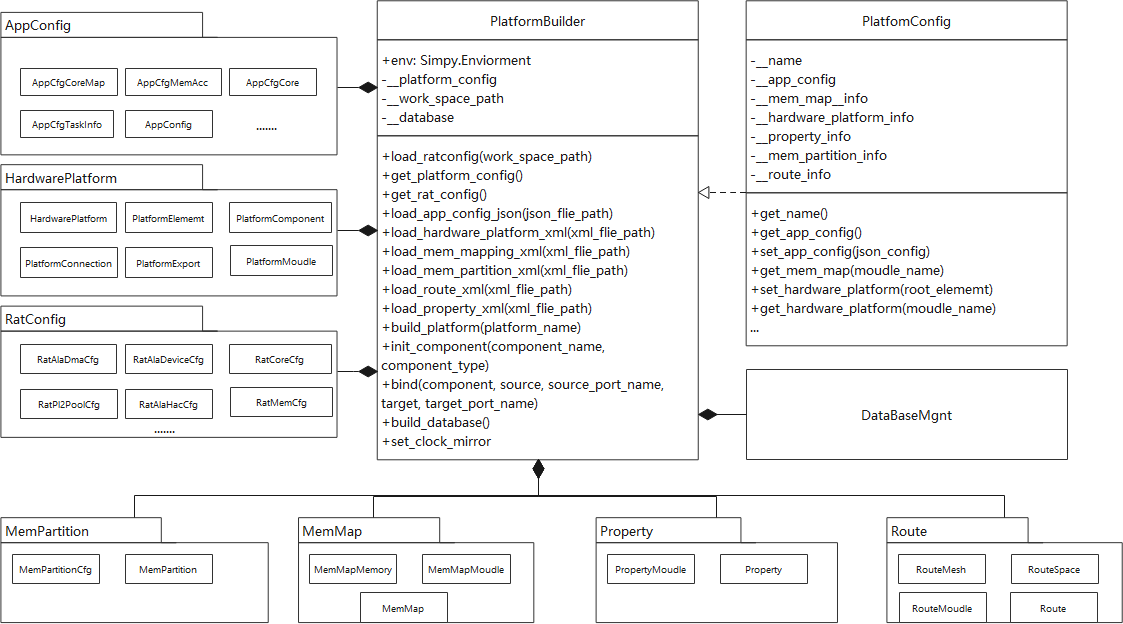
\includegraphics[width=1\textwidth]{硬件模块实例化模块类图.png}
    \caption{硬件模块实例化模块类图}
    \label{fig:badge}
\end{figure}

图5.2硬件平台实例化模块需要的类以及类之间关系构造的类图,在硬件平台实例化
模块中,我们在最外层通过SaeSimulator单实例调用load\_platform函数实现
PlatformBuilder类中对各个硬件配置文件的读取和解析以及实现硬件平台中
各个模型的实例化,PlatformBuilder类读取和解析硬件配置文件后,将硬件
配置信息存储到PlatformConfig类中各个属性中,并对每个属性设置get和
set函数,支持外部对类里面私有函数的设置和读取。最后,硬件模型的实
例化通过调用init\_component函数实现。

硬件模块实例化过程中,实现方式通过层次性的实例化。先按模块解析硬
件配置文件读取硬件配置信息。在逐层实例化各个模块。如硬件模块实例
化类图所示,每个包里是硬件的一部分,将包里的各个类根据读取的硬件
配置信息实例化,在实例化整个次外层的类,如AppConfig里的AppConfig
类。最后在init\_component函数中统一,最后通过bind函数将各个模块
通过路由信息中Port口连接起来。最后,通过DatabaseMgnt类实例化并
连接数据库文件。

\section{GeneralFifo模块设计与实现}

在整个仿真平台中,我们需要实现硬件模型能够在别的模块发送过来消息时
能够及时的对发送过来的消息进行处理,以及模型外部能够接收别的模型发
送过来消息的消息队列。这种消息队列主要用于Processor模块的流水线功能
的具体实现。

我们基于SimPy的事件机制实现了GeneralFifo模块,并在整体仿真平台构建
时将此模块作为基础数据结构使用,与先入先出队列的整体逻辑类似。我们
在概要设计中简要介绍了GeneralFifo的整体执行流程。我们在这一节详细
介绍GeneralFifo的设计。GeneralFifo模块的类图如图5.3所示:
\begin{figure}
    \centering
    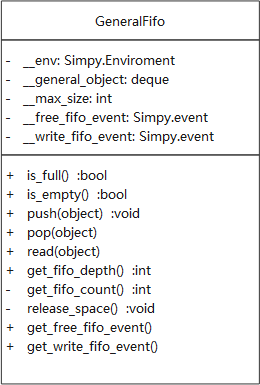
\includegraphics[width=0.45\textwidth]{GeneralFifo类图.png}
    \caption{GeneralFifo类图}
    \label{fig:badge}
\end{figure}

GeneralFifo模块的底层实现基于数据结构双向队列deque实现。整体实现
队列先入先出,并可以设置以及查询队列深度,查询队列中现有对象数量,
判断队列的状态。并基于SimPy的event机制实现了队列的Push和Pop功能。
每次将对象Push进队列时,将触发该队列的write\_fifo\_event,该event事
件触发时,会使在其他模块等待该事件触发的进程开始继续执行,从而实
现该队列一旦有对象存入,能够及时通知其他模块将对象从队列中取出进
行操作。同时,当队列为满时,其他模块只需等待free\_fifo\_event事件
触发,其他模块即可继续向Fifo中Push对象。这样就实现了不同模块之
间基于GeneralFifo的信息传输的功能,以及实现一个进程或者模块等待信息的
场景。在仿真平台中所有模块之间交互以及Processor模块的实现都是
基于GeneralFifo实现的。

\section{Processor模块设计与实现}

仿真平台中Processor模块主要功能为:接收调度器模块发送过来的任务实例并
提取任务实例中中的任务信息,在具体的硬件实例上根据任务信息处理任务。
Processor模型类型主要分为DSP模块、DMA模块和HAC模块。下面详细阐述了
仿真平台Processor相关模块设计与实现。

Processor模块主要实现对三种基础硬件模型(DSP、HAC和DMA)的建模
以及Processor模块与调度器模块之间的交互。在实现三种基础模型的
建模之前,我们实现ProcessorBase类,通过ProcessorBase类所有
Processor模型的基础功能进行实现。

平台中所有模型都是以GeneralModule类为基类实现,GeneralModule
模块是统一所有已实例化的模型并将这些模型联系起来的模块。GeneralModule
模块实现了平台信息和实际硬件模型信息的联系,并为每个模型模块创
建了Log文件,在各模块中可以调用其基类GeneralModule类中的log方
法去记录log信息,并统一设置整个仿真过程中的log等级,以应对不同情
况下的业务仿真;GeneralModule模块中也将数据库模块和具体模块之间
联系起来,在各模块中可以调用其基类GeneralModule类中的message
方法去记录信息并存储到数据库中。

Processor模块具体实现三种模型的功能建模,分别为DMA模型、DSP模型
以及HAC模型。DMA模型的主要功能是要实现数据搬运功能,为DSP模型中
的具体执行将数据从SL2搬运到相应DSP组的PL2中或者数据处理结束后从
PL2搬运到SL2,再或者仅仅只进行内存中的数据交换。DSP模型模拟DSP芯片的
数据处理任务执行过程的流程,主要执行数据的处理。HAC模型模拟了从数据搬
运到数据处理再到数据搬出的整体流程。HAC主要为了执行某一种特定的
执行多次的硬件任务,任务在HAC上执行速度较快,任务的整个执行流程
均在HAC硬件上完成。

% 调度器模块与Processor模块交互以及任务执行整个流程
整个任务执行流程周期是由任务管理模块解析任务实例为开始,任务管理模块解析
任务实例后,由调度器模块接收任务管理模块解析后并重新整理的任务实例,调度器
模块根据接收到的任务信息去申请对应的硬件资源(包括硬件模型以及空闲的内存空间),
接下来调度器模型将任务实例发送到申请到的硬件模型上,由对应的硬件模型对任务实例
进行处理,硬件模型对任务处理完成后,将任务执行完的响应消息发送回调度器,由调度
器模型对该任务实例标记完成,此时一个任务的整个执行流程就结束了。任务实例的整个
执行流程图如图5.4所示:
\begin{figure}
    \centering
    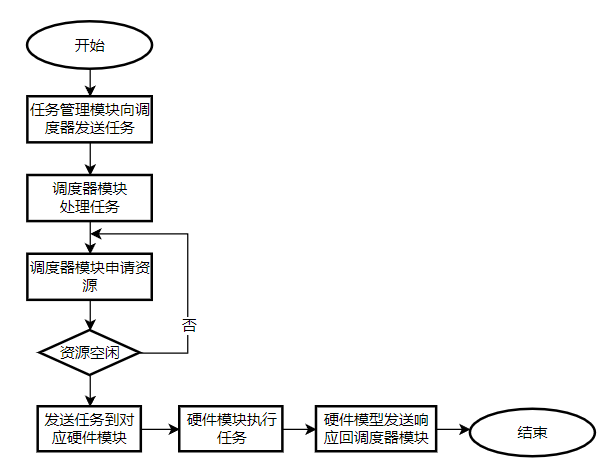
\includegraphics[width=0.8\textwidth]{任务执行流程图.png}
    \caption{任务执行流程图}
    \label{fig:badge}
\end{figure}

调度器模块需要将任务分发到调度器中资源调度模块申请的特定的硬件模型。
但由于整个平台软硬件设计分离,调度器模块无法获取硬件平台整体构
建信息,无法直接与硬件模块之间进行信息交互。因此我们需要一个模块实现调
度器模块与具体硬件模型之间的交互,为此我们在Processor模块中设
计了单实例ProcessorMgnt,用于实现消息交互功能。Processor模块以及
相关模块关系如图5.5所示:

\begin{figure}[!h]
    \centering
    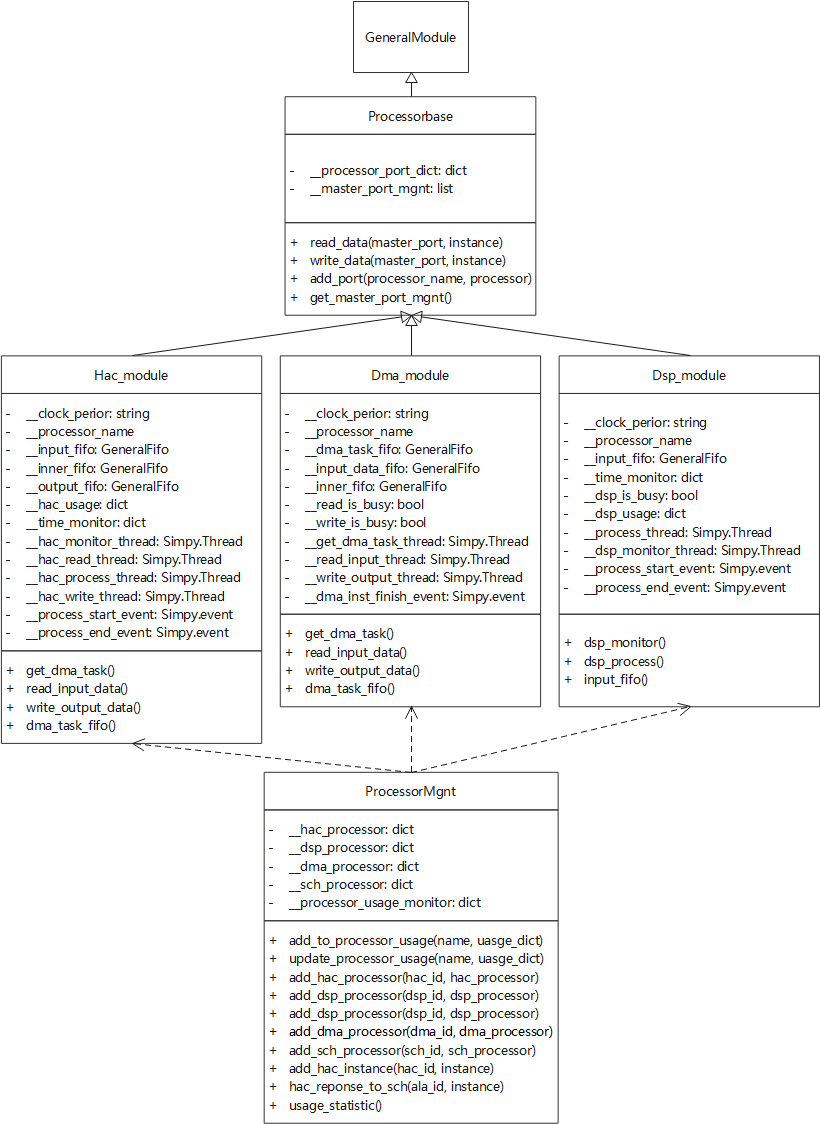
\includegraphics[width=0.8\textwidth]{Processor模块类图.png}
    \caption{Processor模块类图}
    \label{fig:badge}
\end{figure}

图5.5显示了ProcessorMgnt、三种具体的Processor模型、所有
Processor模型的基类ProcessorBase以及几者之间的关系。在
ProcessorMgnt模块中,各个模块在实例化的时候通过调用单实例的
对应方法通过相应类型的dict去记录,dict以模型名为键值。当其
他模块模块之间需要进行交互时,就可以通过调用ProcessorMgnt
单实例相应方法去访问对应字典,通过模型名就可以取到相应的模
型对象,从而进行交互。

三种基础的硬件模型以ProcessorBase为基类。ProcessorBase类实
现了几种基础硬件模型的公有方法:如实例化Port、读数据、写数
据、管理MasterPortMgnt等等。在介绍具体的Processor模型实现之前,
我们先介绍在仿真平台中传输的数据类型。

在仿真平台中传输的数据主要包括RwObject、Burst以及Flit三种。在
最外层硬件模块中传输数据的数据类型为RwObject,数据在总线上
传输的数据格式为Flit。这三种数据格式均包含着数据请求的关键信息:
请求类型、目的地址,数据长度等等,还包含着每个对象独有的id(如ObjectId,
BurstId等等)。DMA模块或者HAC模块需要进行数据搬运的时候,
将数据封装成RwObject发送到所在硬件对应的Port上,由PortMgnt模块
对RwObject进行拆分,将其拆分成总线位宽的Flit数据帧。Flit数据帧
仅在总线上可见,在仿真平台上可见的还是RwObject。图5.6为三种数据
类型的类图,以及图5.7为三种数据类型之间的关系图。
\\
\\
\\

\begin{figure}
    \centering
    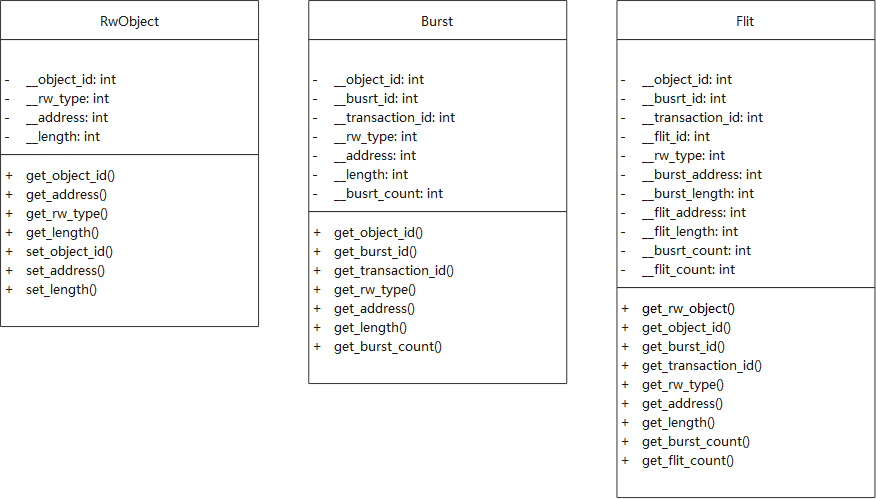
\includegraphics[width=1\textwidth]{三种数据类型类图.png}
    \caption{三种数据类型类图}
    \label{fig:badge}
\end{figure}

\begin{figure}
    \centering
    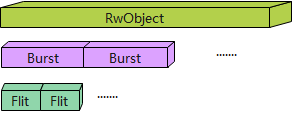
\includegraphics[width=0.6\textwidth]{数据类型关系图.png}
    \caption{数据类型关系图}
    \label{fig:badge}
\end{figure}


下面介绍三种基础硬件模型的具体实现:首先我们介绍DSP模块
的功能实现。DSP模块模拟的是DSP芯片的数据处理任务执行过程,在
仿真平台的流程中只需模拟真实的处理时延即可。调度器模块将任务用
例通过ProcessorMgnt模块发送到DSP模块的input\_fifo中,在硬件模
型中process\_thread一直在等待输入,DSP模型的input\_fifo中一旦有对象传入,
该事件被触发后,process\_thread进程就开始进行处理。处理时延在输入的任务
描述符中已经存在,DSP模型只需从任务描述符中取出时延信息,在乘以硬件的时钟
频率即可得到需要等待的仿真时间。DSP模块在任务链中作用负责完成输入数据的处理。
在仿真平台中只完成处理时延的仿真,并不真实的进行数据的处理。前搬移任务、DSP任
务以及后搬移任务形成一整个任务链,三者任务信息由同一个任务实例携带,当前搬移
DMA任务完成时,解析任务实例中的信息得到下一级DSP任务的硬件模型名,通过
ProcessorMgnt将任务实例发送到对应DSP模型input\_fifo中,触发相应的DSP任务,
发回调度器的响应只用来释放DMA任务申请的系统资源。

接下来介绍DMA模块的功能实现。在仿真平台中,DMA任务一般分为纯DMA任务、前搬移
任务以及后搬移任务。其中前搬移任务和后搬移任务都是包含在DSP任务链里面的,而
纯DMA任务只是单纯将数据从一块地址搬移到另外一块地址。DMA模块需要完成的对DSP
模块需要进行处理的数据的搬入搬出,将数据从对应SL2内存中搬入DSP模
块的PL2内存中的过程称为前搬移,将数据从PL2内存搬运到SL2
的过程称为后搬移。数据的搬入搬出,DMA模块通过任务用例中
的地址和数据大小信息创建RWObject,通过MasterPortMgnt经
过总线进行传输,DMA模块在实例化的过程中创建两个线程分别用来处理数据的搬入和
数据的搬出,以及创建一个线程获取DMA任务实例和控制总体
的流水线深度。DMA模块通过各级线程以及线程之间的Fifo实
现流水线。每一级线程均从Fifo中取出任务实例,执行完任务
实例之后,再将任务实例发到下一级线程的Fifo中,从而实现流水线
。DMA模块的流水线执行时序图如图5.8所示:

\begin{figure}
    \centering
    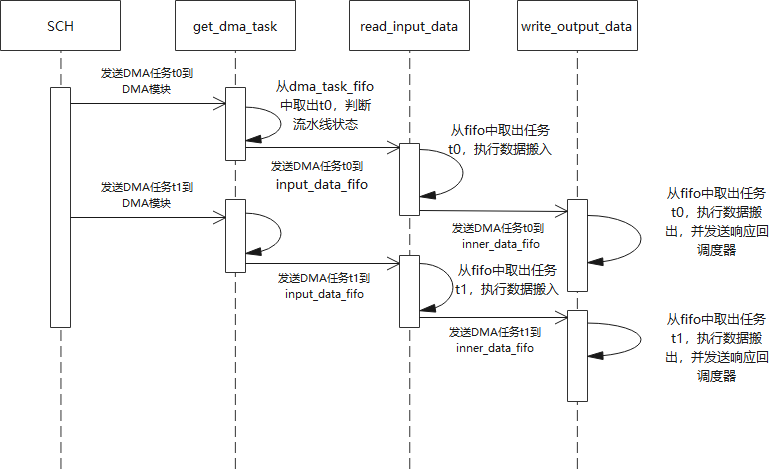
\includegraphics[width=1\textwidth]{DMA模块流水线时序图.png}
    \caption{DMA模块流水线时序图}
    \label{fig:badge}
\end{figure}


HAC模块是用来处理专用任务的硬件。一种HAC只用来执行一种任务,用来加速任务的处理。
HAC硬件模块中需要完成数据的搬入、处理以及搬出的一整套流程。HAC模块接收调度器
模块发送过来的HAC任务实例,HAC任务实例中记录着输入数据、处理时延以及输出数据等
相关信息。HAC模块通过三级流水实现数据搬入、数据处理以及数据搬出的功能。调度器模块
发送HAC任务实例到相应HAC模块的input\_fifo中,当input\_fifo接收到任务实例后,
HAC模块的input\_thread等待的事件被触发,进程加锁不再接收任务实例,进程开始执行
数据搬入的操作,把数据从相应的SL2内存中搬运到PL2内存中,操作执行结束后,将任务实例
放入inner\_fifo中,进程解锁。后续两个进程重复此类操作,形成HAC内部的三级流水的任务
执行。HAC模块的三级流水时序图如图5.9所示:

\begin{figure}
    \centering
    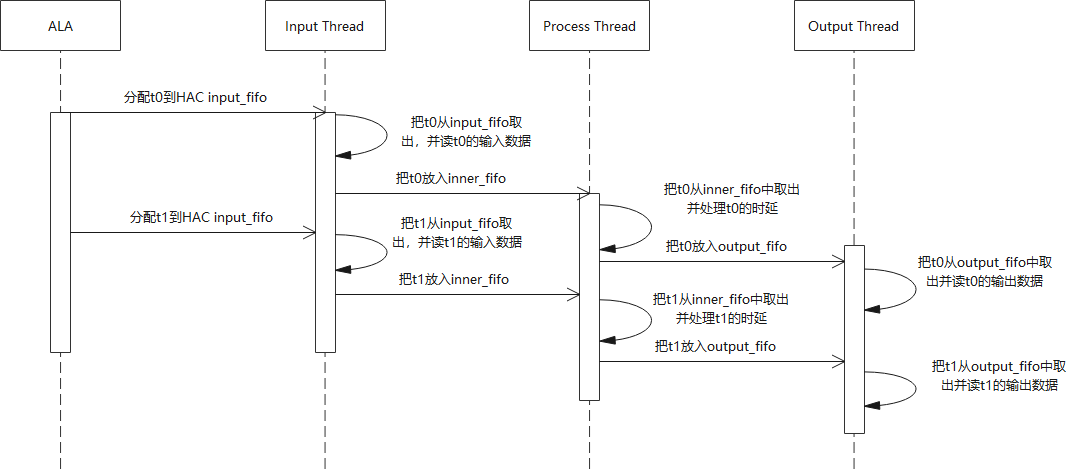
\includegraphics[width=1\textwidth]{HAC模块三级流水时序图.png}
    \caption{HAC模块三级流水时序图}
    \label{fig:badge}
\end{figure}

此外,Processor模块还在DSP模型和HAC模型中实现统计每个定长的时间片
内的硬件利用率。通过dsp\_monitor\_thread和hac\_monitor\_thread
两个进程分别去统计DSP模型和HAC模型的执行时间片。以DSP模块
为例,DSP模块在从FIFO中取出任务实例时触发process\_start\_event,
处理完时延后触发process\_end\_event。这两个事件都会使挂起的进程
开始执行,从而统计DSP模型每次执行的时间片区间。同时为了统计每一段
时间片内每个硬件的占用率,硬件模型中ProcessorMgnt模块统计了所有硬件模型的
对象,ProcessorMgnt模块在平台初始化时创建processor\_usage\_monitor字典,
processor\_usage\_monitor每个时间片的每个硬件模型的核利用率初始值设置为0,用于
统计每段时间片内的硬件利用率,并在对应的硬件模型中通过对应的进程去记录。在相应
的进程中,先设置变量Start和End来记录任务的开始时间戳以及结束时间戳,并设置标记
记录当前时间戳为任务开始的时间戳还是任务结束的时间戳。并通过每次Start和End之间时
间差去计算统计每个时间片的硬件利用率,并将相应的核利用率记录到processor\_usage\_monitor
中。在整个用例仿真结束后,在ProcessorMgnt模块中通过usage\_statistic方法去将
processor\_usage\_monitor中的内容统一的存储到数据库中。HAC模型内部工作时间块
统计与之相同。硬件模型核利用率的监控进程的算法图如图5.10所示:
\\
\\
\\
\\
\\
\begin{figure}
    \centering
    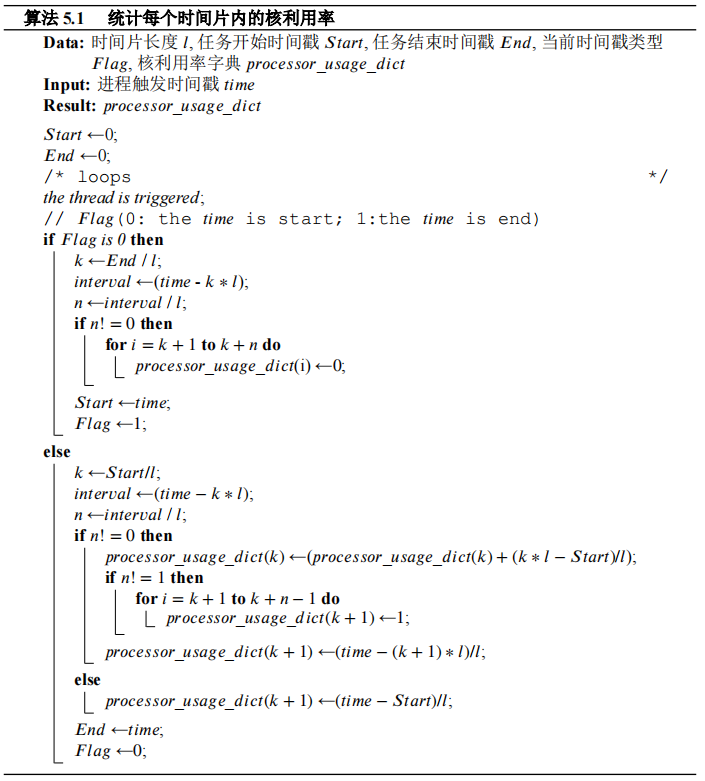
\includegraphics[width=1\textwidth]{Processor监控进程算法图.png}
    \caption{Processor监控进程算法图}
    \label{fig:badge}
\end{figure}

\section{仿真平台Memory模块设计与实现}

仿真平台的Memory模块主要实现接收Master设备通过总线互联模块发送
过来的读写请求flit,根据Bank位宽拆成对应的Bank操作发送到对应地
址的Bank的FIFO上。

Memory模块提供交织的Bank。这些Bank模块根据地址相互交织,每个Bank
的偏移地址与Bank位宽相同。仿真平台中Memory模块Bank模块设计为4个Bank,
Bank位宽为256字节的设计方案。Memory模块在实例化的时候创建4个Bank模块,
Memory模块可以同时处理不同的Bank模块上的Bank操作,但每个Bank模块同时只
能处理一个Bank操作。Bank模块的交织方案如图5.11所示:
\begin{figure}
    \centering
    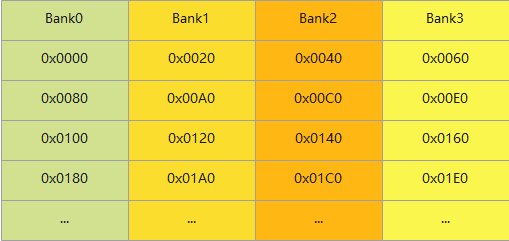
\includegraphics[width=0.82\textwidth]{Bank模块交织方案.png}
    \caption{Bank模块交织方案}
    \label{fig:badge}
\end{figure}

Bank模块在初始化时创建读写Bank线程。读写Bank操作完成向对应的SlavePort
发送读写响应flit。Memory模块接收SlavePort发送过来的flit,因为对读写请
求的操作不同,Memory模块会根据读写请求的区别分到不同的FIFO中。Memory对
发送过的flit的处理流程图如图5.12所示:

\begin{figure}
    \centering
    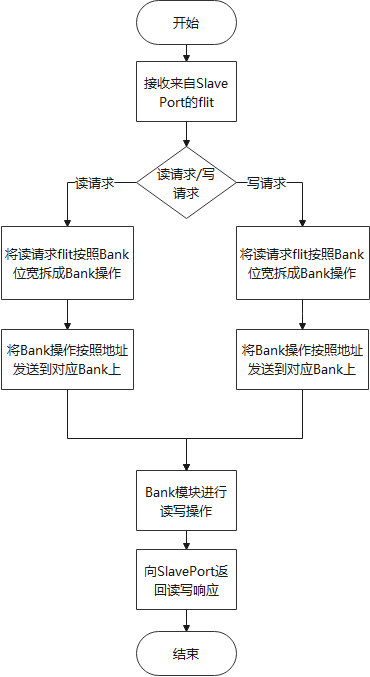
\includegraphics[width=0.49\textwidth]{Memory模块处理流程图.png}
    \caption{Memory模块处理流程图}
    \label{fig:badge}
\end{figure}

Bank写操作结束时,Memory模块会统计一个Burst完成flit的数量,当最后一个flit
操作完成后会统一发送一个写响应回SlavePort。而Bank读操作则时完成一个flit就
发送一个flit的读响应到SlavePort上。最后由总线互联模块发送回发送读写请求的
Master设备,完成一整个读写操作。

\section{设计空间探索相关模块的设计与实现}

设计空间探索模块实现的功能是对我们所需要探索的设计目标在设计空间中寻找最优
或者是较优设计。设计空间模块主要分为三个模块:训练集生成模块、预测模型生成
模块以及遗传算法探索模块。设计空间探索模块的整体流程图如图5.13所示:

\begin{figure}
    \centering
    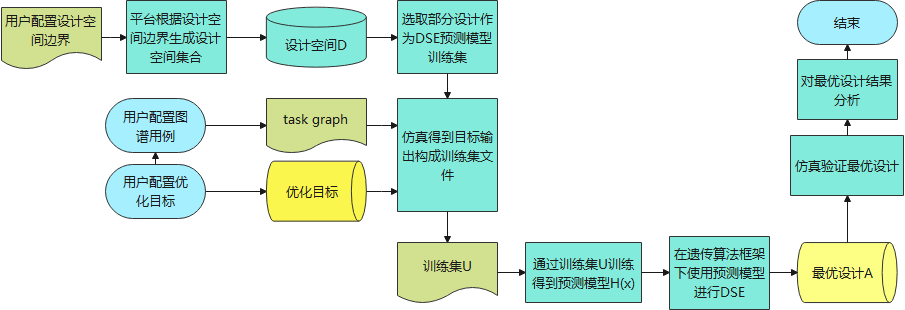
\includegraphics[width=1\textwidth]{设计空间探索模块整体流程图.png}
    \caption{设计空间探索模块整体流程图}
    \label{fig:badge}
\end{figure}

接下来主要介绍训练集生成模块和预测模型生成模块的具体设计与实现以及设计空间探索结果分析。

\subsection{训练集生成模块的设计与实现}

训练集生成模块主要包括设计参数、设计边界与目标值的选取、设计空间的生成以及根据设计空间
以及目标值生成下一步预测模型所需要的训练集文件。在仿真平台中我们选取可配置参数作为我们
的设计参数,并根据实际情况设置各个设计参数的设计边界,具体设计参数及设计边界如表5.1所示:

\begin{table}[!h]
    \centering\normalsize
    \caption{仿真平台设计空间}
    \begin{tabular}{c|c|c}
    \hline
    \textbf{设计参数} & \textbf{设计参数取值}         & \textbf{数量} \\ \hline
    PL2 Pool Size & 100000-190000: 10000+   & 19          \\ \hline
    PL2 Unit Size & 10-50: 10+              & 5           \\ \hline
    SL2 Pool Size & 1500000-1850000: 50000+ & 7           \\ \hline
    SL2 Pool Size & 10-50: 10+              & 5           \\ \hline
    Cu Num        & 1-5: 1+                 & 5           \\ \hline
    Dsp Num       & 4-16: 2+                & 7           \\ \hline
    BUS Bit Width & 64-512: 64+             & 8           \\ \hline
    \end{tabular}
    \end{table}

我们选取了七个参数作为我们设计空间探索的设计参数值,设计参数分别为:PL2内存池大小、PL2每个内存单元大小、SL2内存池大小、SL2每个内存单元大小、Cu数量、Dsp数量以及总线位宽。这些参数均会影响最后仿真结果。这些设计参数的组合最后构成的设计空间包括了超过56万个不同的设计配置。

我们设计空间探索主要探索的方向主要是时延以及核的使用方面。我们最终选取了仿真时延、每个TTI核的利用率、每个TTI核的一致性为我们设计空间探索的目标值。接下来我们说明每个目标值的统计标准。仿真时延在数据库文件中有着直接的记录,我们只需直接提取数据库中的信息即可,核的利用率在数据库中记录了每个时间片(0.002TTI)的核的利用率,记录方法已在5.1.5节介绍。我们只需将数据库中信息整合每个TTI的核的利用率即可。核的一致性指的是在同个TTI内所有核的利用率的方差,我们需要将之前统计的核的利用率进行计算即可。这就是我们设计空间探索的优化目标值。

我们生成训练集的流程图如图4.9所示。我们将RatConfig表中需要改变的参数值单独设置一页Config
表,并将这一页的值与整张表中的相关的值相关联,通过openpyxl插件去修改Config表中的参数。
这样我们就可以通过脚本自动改变设计参数去运行仿真,仿真结束后提取数据库中目标值信息,处理
后将设计参数和目标值一同输出到训练集文件中。我们训练集文件大小为6000,生成训练集模块一共
运行了6000次仿真。训练集文件格式如图5.14所示:

\begin{figure}
    \centering
    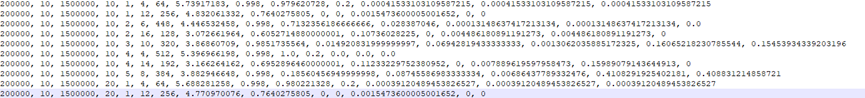
\includegraphics[width=1\textwidth]{训练集文件格式示例.png}
    \caption{训练集文件格式示例}
    \label{fig:badge}
\end{figure}

\subsection{预测模型生成模块设计与实现}

我们在遗传算法进行设计空间探索过程中,在不断迭代每一代种群时如果每一次都要进行仿真从而得到对应设计参数的目标值,整体设计空间探索的时间就会十分的漫长。于是,我们使用机器学习生成的预测模型去代替实际的仿真平台去进行遗传算法设计空间探索的过程,这样能够大大减少设计空间探索的时间。

我们多目标预测模型采用先对不同目标值分别进行机器学习的过程,得到对应7个目标值的7个预测模型。我们将这7个预测模型通过一个multi\_model类集成到一起,通过multi\_model类的方法我们可以通过输入设计参数从而得到相应的目标值。多目标预测模型集成的各个目标值的准确度(以R2确定系数为标准)如表5-2所示:

\begin{table}[!h]
    \centering\normalsize
    \caption{多目标预测模型误差值}
    \begin{tabular}{|c|c|c|c|}
    \hline
    \textbf{时延}       & \textbf{TTI0核利用率} & \textbf{TTI1核利用率} & \textbf{TTI2核利用率} \\ \hline
    0.99824568        & 0.9999998         & 0.9982341         & 0.9873023         \\ \hline
    \textbf{TTI0核一致性} & \textbf{TTI1核一致性} & \textbf{TTI2核一致性} & \textbf{}         \\ \hline
    0.8638929         & 0.9831229         & 0.8559540         &                   \\ \hline
    \end{tabular}
    \end{table}

从表中我们可以清楚的看出对于多个目标值而言,每个目标值的误差值不超过0.15。整个预测模型可以
比较高效精准的预测出目标值,与真实仿真平台的仿真结果相差不大,为了更加精准的看出预测模型
与仿真平台的结果差距,我们将1200次仿真结果作为验证集与预测模型进行对比,仿真结果与预测结果
对比如图5.15所示:

\begin{figure}[!h]
    \centering
    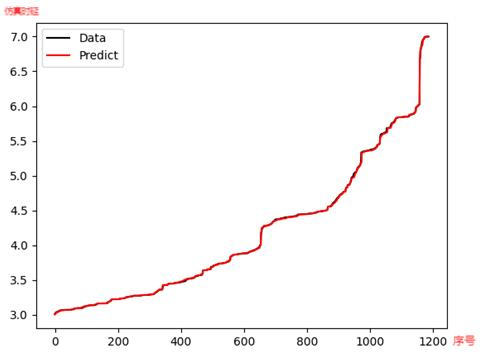
\includegraphics[width=0.45\textwidth]{仿真结果与预测结果对比图1.png}
\end{figure}

\begin{figure}[!h]
    \centering
    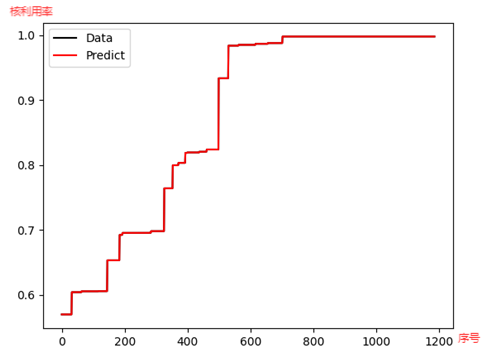
\includegraphics[width=0.45\textwidth]{仿真结果与预测结果对比图2.png}
\end{figure}

\begin{figure}[!h]
    \centering
    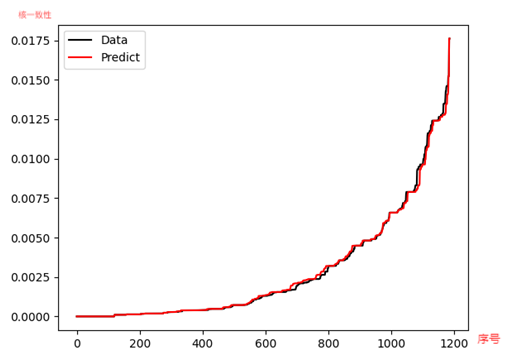
\includegraphics[width=0.45\textwidth]{仿真结果与预测结果对比图3.png}
    \caption{仿真结果与预测结果对比图}
\end{figure}

\subsection{设计空间探索结果分析}

在得到多目标预测模型之后,我们将使用多目标预测模型使用遗传算法进行设计空间探索。遗传算法执行过程中我们
使用NGSA-Ⅱ,我们通过交叉变异等操作产生子代,将父代和子代放到一起进行快速非支配排序,构造出不同等级
的非支配解集。按照需求计算每一代所有个体的拥挤距离,并根据拥挤度比较构造下一代种群。

遗传算法我们遗传代数设置为200代,每代种群数量为50,变异概率为0.1。最终演化种群中的每个基因型经过仿真平
台仿真运行得出相应的目标值。最终我们得到了50个设计方案,并且将这50个设计方案在仿真平台上进行仿真,得到
了相应的目标值。我们根据这50个设计方案以及对应的目标值进行探索,得到了以下结论。

我们先将三个方面的50个目标值与原始设计相对比得到图5.16。

\begin{figure}
    \centering
    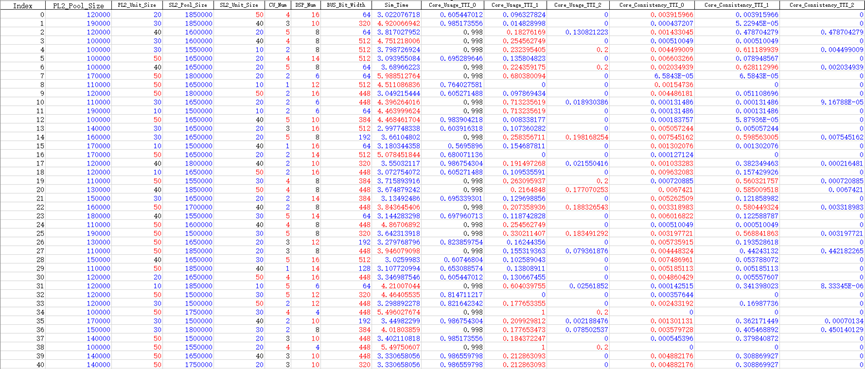
\includegraphics[width=1\textwidth]{设计空间探索结果仿真目标值结果对比图.png}
    \caption{设计空间探索结果仿真目标值结果对比图}
    \label{fig:badge}
\end{figure}

根据图5.16针对仿真时延、核利用率以及核一致性三个目标值,我们可以得到相
对于这三个目标值各自方向的最优解。下面我们对三个目标值单独进行分析并将
设计空间探索所得到的最优解集放在一起进行比较。我们基于优化目标将所有方
案的结果以及原始设计方案放到一起进行比较。比较结果如图5.17至5.19所示:

\begin{figure}[h]
    \centering
    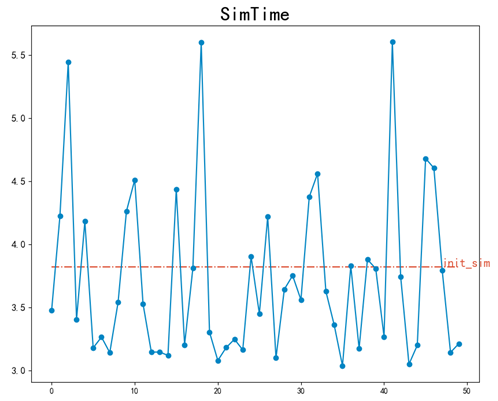
\includegraphics[width=0.53\textwidth]{50组设计方案时延结果对比.png}
    \caption{50组设计方案时延结果对比}
    \label{fig:badge}
\end{figure}

图5.17中横坐标为设计方案序号,纵坐标为仿真时延,红色虚线为初始设计方案及其对应的仿真时延。
由图5.17及对应序号的设计方案可以看出序号为35、43、20、27、14、7、48、12、13、23的方案较好。
并且通过各个设计方案值之间的结果对比可以得出影响时延结果的主要因素为核的数量以及总线位宽等等。
\begin{figure}[h]
    \centering
    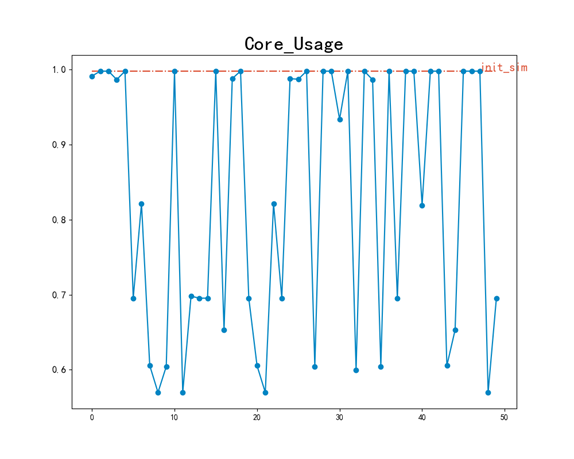
\includegraphics[width=0.6\textwidth]{50组设计方案核利用率结果对比.png}
    \caption{50组设计方案核利用率结果对比}
    \label{fig:badge}
\end{figure}

由图5.18及对应序号的设计方案可以看出序号33、28、42、29、47、39、36、38、4、26的方案较好。
并且通过各个设计方案之间的结果对比可以得出影响核利用率的主要因素为核的数量及CU数量等等。

\begin{figure}[h]
    \centering
    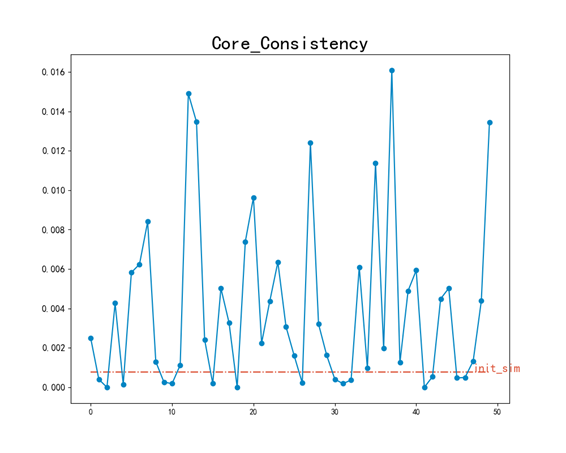
\includegraphics[width=0.6\textwidth]{50组设计方案核一致性结果对比.png}
    \caption{50组设计方案核一致性结果对比}
    \label{fig:badge}
\end{figure}

由图5.19及对应序号的设计方案可以看出序号2、18、41、4、31、15、10、26、9、32的方案较好。
并且通过各个设计方案之间的结果对比可以得出影响核利用率的主要因素为核的数量及CU数量等等。
而且对比图5.17和图5.18可以发现核利用率和核一致性的优化方向和影响因素大致相同。

但针对多个目标值同时考虑而言,我们需要找到多个目标值均衡的几个设计方案。从图5.16至图5.18可以看出
时延和核的利用率优化方向相反。仿真时延低的几种方案,设计参数中Dsp数量较大,但由于Dsp数量较大,
导致核的利用率和一致性效果较差。而核的利用率和核的一致性优化方向相同,最优的几个设计方案设计参数
大致相同。于是我们就核利用率和仿真时延两个方面进行考虑,结果图如图5.20所示:
\\
\\
\begin{figure}[h]
    \centering
    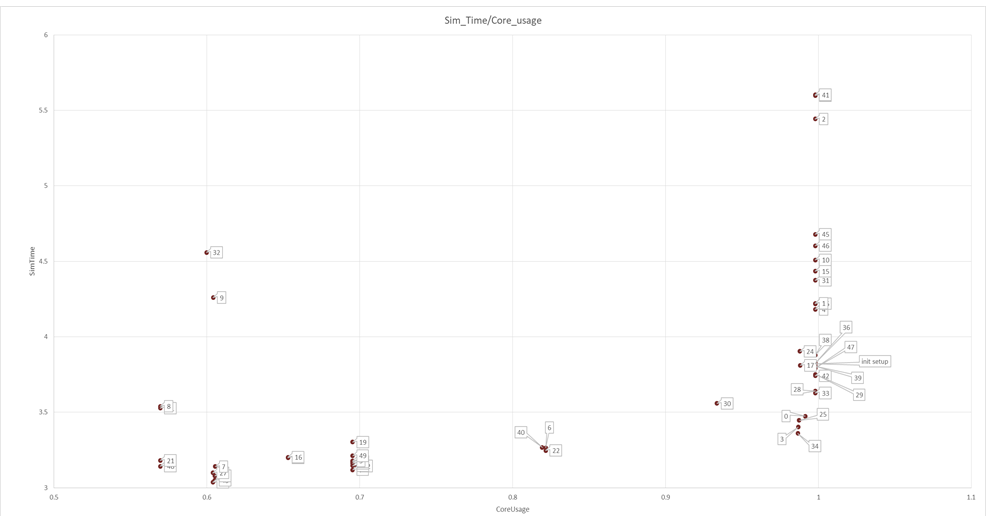
\includegraphics[width=1\textwidth]{仿真平台结果分析图.png}
    \caption{仿真平台结果分析图}
    \label{fig:badge}
\end{figure}

从图5.20中我们可以找到6种方案在仿真时延和核利用率两个方面表现都很优秀的设计方案如表5.3所示:

\begin{table}[h]
    \centering\footnotesize
    \caption{最优设计方案设计参数}
    \begin{tabular}{|c|c|c|c|c|c|c|c|}
    \hline
    Index & PL2\_Pool\_Size & PL2\_Unit\_Size & SL2\_Pool\_Size & SL2\_Unit\_Size & Cu\_Num & Dsp\_Num & BUS\_Bit\_Width \\ \hline
    33    & 140000          & 30              & 1550000         & 20              & 4       & 8        & 448             \\ \hline
    25    & 170000          & 40              & 1650000         & 10              & 5       & 10       & 320             \\ \hline
    3     & 170000          & 20              & 1800000         & 50              & 2       & 10       & 512             \\ \hline
    42    & 100000          & 20              & 1800000         & 20              & 4       & 8        & 512             \\ \hline
    0     & 100000          & 10              & 1750000         & 50              & 4       & 10       & 128             \\ \hline
    25    & 170000          & 30              & 1650000         & 10              & 5       & 10       & 320             \\ \hline
    \end{tabular}
    \end{table}

从整体设计参数以及目标值的变化,我们可以看出增加Cu数量可以增快仿真速度,提高总线带宽可以使核的利用率提高同时还可以增快仿真速度。

\section{本章小结}

本章的工作主要是在第四章概要设计的基础上,详细的阐述了仿真平台中硬件平台
的构建、Processor模块以及Memory模块的具体实现,介绍了设计空间探索流程的
具体设计和实现。实现整个仿真平台的搭建以及基于仿真平台的设计空间探索流程,
最后得到了设计空间探索结果种群,并对最终得到的设计空间探索结果进行了分析,得到了最终的
最优设计方案以及设计方案优化的目标

在本章基础上,下一章节将详细阐述对仿真平台的测试。
% !TeX root = ../main.tex

\chapter{系统测试与结果分析}

本章主要针对系统对仿真平台的仿真平台的需求,对整个仿真平台进行功能性和非功能性测试。
\section{仿真平台测试}

\subsection{测试环境}

因为公司项目的保密性,所有测试环节均在公司电脑上完成,测试电脑的配置如下所示:

CPU::Intel(R) Core(TM) i7-8700 CPU @3.2GHz

内存:32G

磁盘:1T

操作系统:Windows10

系统类型:64位操作系统

\subsection{测试工具和方法}

针对仿真平台,测试主要包括功能测试和非功能测试两个部分。功能测试主要从两个
方面进行测试,一方面,在整个平台构建之前,我们需要对建模好的各个硬件实例进行
功能测试,保证其功能正确。另一方面,在所有模块单独测试通过后,在整个仿真平台
构建时,我们从程序的输入输出为角度,对仿真平台的各个模块进行测试。这里主要对
硬件平台构建模块和仿真运行模块这两个模块的功能进行测试。针对仿真平台而言,我
们需要得到有效的仿真结果,包括时延、任务的开始结束信息、内存信息以及核的使用
情况等等。且仿真平台需要保证任务仿真执行时序与任务用例图的时序一致。

\subsection{硬件模块功能测试}
在对各个建模好的硬件模块进行功能测试主要测试的是实例化后的硬件模块时候能够
接收来自其他模块的消息并即时触发执行任务的流程、自身的硬件功能以及能够正常
与其他模块进行消息交互。在这个测试过程中,我们主要对GeneralFifo模块、Processor
模块以及Memory模块这三个模块进行测试。针对需求分析中对这三个模块提出的测试
指标进行测试,测试结果如表6.1、表6.2和表6.3所示:

\begin{table}[]
    \centering
    \caption{GeneralFifo模块测试表}
    \begin{tabular}{|c|c|c|c|c|}
    \hline
    \textbf{序号} & \textbf{测试项}                                             & \textbf{操作流程}                                                                    & \textbf{预测结果}                                             & \textbf{实际结果} \\ \hline
    1           & \begin{tabular}[c]{@{}c@{}}能否正确的\\ 存取对象\end{tabular}     & \begin{tabular}[c]{@{}c@{}}调用GeneralFifo的方法\\ 函数来存取对象\end{tabular}               & \begin{tabular}[c]{@{}c@{}}通过调用函数方法\\ 成功存取对象\end{tabular} & 正确            \\ \hline
    2           & \begin{tabular}[c]{@{}c@{}}存取函数能否\\ 触发事件\end{tabular}    & \begin{tabular}[c]{@{}c@{}}调用该模块的事件接口\\ 去执行计数任务,存取对象后看\\ 每一步计数值是否正确\end{tabular} & 每一步计数值正确                                                  & 正确            \\ \hline
    3           & \begin{tabular}[c]{@{}c@{}}该模块外部\\ 接口方法是否正确\end{tabular} & \begin{tabular}[c]{@{}c@{}}通过存取对象,调用方法函数,\\ 观察结果是否正确\end{tabular}                & 结果正确                                                      & 正确            \\ \hline
    \end{tabular}
    \end{table}

如表6.1所示,我们对GeneralFifo模块进行了功能性测试,主要分为三个部分,测试项1
测试GeneralFifo模块作为一个先入先出队列的存取对象的功能,通过该模块提供的外部接口
方法,调用函数进行对象的存取,测试结果表示该功能正确。

测试项2测试GeneralFifo的事件机制是否能够被正确触发,GeneralFifo模块提供内部的event
事件接口,其他模块可以通过Simpy的yield机制去等待该event被触发。我们通过设置计数任务,每次
event被触发,计数任务被触发且打印计数值,我们通过像队列中存取对象来触发对象,
通过观察计数值,即可测试出GeneralFifo模块的事件机制是否正确。最后测试结果
表明GeneralFifo模块的事件机制正确。

测试项3测试GeneralFifo模块提供外部接口和方法是否正确,这部分我们只需通过调用
模块的外部接口即可测试,通过这部分测试表明GeneralFifo模块的外部接口正确。

\begin{table}[]
    \centering
    \caption{Processor模块测试表}
    \begin{tabular}{|c|c|c|c|c|}
    \hline
    \textbf{序号} & \textbf{测试项}                                                        & \textbf{操作流程}                                                                    & \textbf{预测结果}                                                    & \textbf{实际结果} \\ \hline
    1           & \begin{tabular}[c]{@{}c@{}}DSP模块处理能否\\ 即时并准确的\\ 接收任务实例\end{tabular} & \begin{tabular}[c]{@{}c@{}}向DSP模块入口Fifo发\\ 送任务实例,观察DSP模块\\ 对任务实例的解析\end{tabular} & \begin{tabular}[c]{@{}c@{}}DSP模块即时接\\ 收并正确解析\\ 任务实例\end{tabular} & 正确            \\ \hline
    2           & \begin{tabular}[c]{@{}c@{}}DSP任务处理时延\\ 是否与任务实例\\ 中一致\end{tabular}   & \begin{tabular}[c]{@{}c@{}}DSP接收并处理\\ 任务结束,查看\\ 仿真环境的时延\end{tabular}             & \begin{tabular}[c]{@{}c@{}}仿真环境的时延\\ 变化与任务实例\\ 中一致\end{tabular}  & 正确            \\ \hline
    3           & \begin{tabular}[c]{@{}c@{}}DMA模块处理能否\\ 即时并准确的\\ 接收任务实例\end{tabular} & \begin{tabular}[c]{@{}c@{}}向DMA模块入口Fifo发\\ 送任务实例,观察DMA模块\\ 对任务的解析\end{tabular}   & \begin{tabular}[c]{@{}c@{}}DMA模块即时接\\ 收并正确解析\\ 任务实例\end{tabular} & 正确            \\ \hline
    4           & \begin{tabular}[c]{@{}c@{}}DMA模块能否根据\\ 任务信息正确\\ 搬入搬出数据\end{tabular} & \begin{tabular}[c]{@{}c@{}}DMA执行完数据搬\\ 运任务,查看源地址与\\ 目的地址的内存变化\end{tabular}       & \begin{tabular}[c]{@{}c@{}}源地址与目的地址\\ 内存接收数据请求\end{tabular}      & 正确            \\ \hline
    5           & \begin{tabular}[c]{@{}c@{}}DMA模块与DSP\\ 模块能否流水\\ 线化执行任务\end{tabular} & \begin{tabular}[c]{@{}c@{}}向DMA模块发送任务实\\ 例观察整个任务能够\\ 完整执行\end{tabular}           & \begin{tabular}[c]{@{}c@{}}整个任务链完整\\ 且正确的执行\end{tabular}         & 正确            \\ \hline
    6           & \begin{tabular}[c]{@{}c@{}}HAC模块处理能否\\ 即时并准确的\\ 接收任务实例\end{tabular} & \begin{tabular}[c]{@{}c@{}}向HAC模块入口Fifo发\\ 送任务实例,观察HAC模块\\ 对任务实例的解析\end{tabular} & \begin{tabular}[c]{@{}c@{}}HAC模块即时接\\ 收并准确解析任\\ 务实例\end{tabular} & 正确            \\ \hline
    7           & \begin{tabular}[c]{@{}c@{}}HAC模块能否正\\ 确执行任务实例\end{tabular}          & \begin{tabular}[c]{@{}c@{}}HAC执行完整个任务实例\\ ,从对应HAC的日志中提\\ 取任务执行信息\end{tabular}    & \begin{tabular}[c]{@{}c@{}}任务执行信息与任\\ 务实例中信息一致\end{tabular}      & 正确            \\ \hline
    \end{tabular}
    \end{table}

如表6.2所示,我们对Processor模块的三种硬件模型进行了功能性测试。主要按照不同的硬件
模型分为三部分:

测试项1和测试项2主要测试DSP模块的硬件功能是否正确。测试项1通过构造测试用的任务实例,
并将测试用例发送到DSP模块的入口Fifo上,这部分测试当DSP模块的入口Fifo接收到任务实例
时,能不能立即处理任务实例,并能够正确的将任务实例中的任务信息解析出来;测试项2在
测试项1的基础上,测试了DSP模块处理任务实例,任务是否能够被正确执行,DSP任务只体
现时延的变化,只要保证在任务执行结束后,仿真环境的仿真时延变化与任务实例中信息一致
即可。从两项测试的结果来看,DSP模块的硬件功能符合要求。

测试项3\textasciitilde 5主要测试了DMA模块的硬件功能以及DMA模块和DSP模块流水线执行任务的能力。
测试项3通过构造测试用的任务实例,将测试用例发送到DMA模块的入口Fifo上,DMA模块
能够立即取出任务实例并正确的解析任务实例中的任务信息;测试项4在测试项3的基础上
对DMA模块对任务实例的处理能力进行测试,DMA模块负责数据的搬入搬出,我们只需要查看
源地址与目的地址对应的内存模块查看是否收到来自DMA的数据请求;测试项5是测试DMA模块
和DSP模块的流水线执行任务链的能力,在业务场景中常常会出现数据搬运后立即对数据进行
处理的场景,为了满足这种业务场景,测试项5通过构造带有数据搬运以及数据处理的任务链
级的任务实例,观察DMA模块执行完数据搬运能否通知目标DSP实例去执行数据处理任务。根据
测试结果显示,DMA模块的硬件功能以及DMA模块和DSP模块流水线执行任务的能力符合要求。

测试项6和测试项7主要测试HAC模块对任务的处理能力,测试项6通过构造在HAC模块上处理
的特定任务实例,HAC模块能能够立即接收任务实例并且正确的解析出任务实例中的任务信息;
测试项7通过查看对应HAC的日志去提取HAC模块在执行测试用例时的具体任务信息,通过任务
的执行信息,我们从时延变化、数据搬运等方面可以看出任务有没有正确执行。从两个测试项
的测试结果可以看出HAC模块对任务实例的处理能力符合要求。

\begin{table}[]
    \centering
    \caption{Memory模块测试表}
    \begin{tabular}{|c|c|c|c|c|}
    \hline
    \textbf{序号} & \textbf{测试项}                                                 & \textbf{操作流程}                                                          & \textbf{预测结果}                                                  & \textbf{实际结果} \\ \hline
    1           & \begin{tabular}[c]{@{}c@{}}能否正确的\\ 接收读写\\ 数据请求\end{tabular}  & \begin{tabular}[c]{@{}c@{}}发送读写数据请求\\ 到入口Fifo上,\\ 观察其解析结果\end{tabular} & \begin{tabular}[c]{@{}c@{}}解析结果\\ 正确\end{tabular}              & 正确            \\ \hline
    2           & \begin{tabular}[c]{@{}c@{}}能否正确的\\ 处理读写\\ 数据请求\end{tabular}  & \begin{tabular}[c]{@{}c@{}}查看对应模块日志文\\ 件中的数据处理信息\end{tabular}          & \begin{tabular}[c]{@{}c@{}}数据处理信息\\ 与数据请求中\\ 信息一致\end{tabular} & 一致            \\ \hline
    3           & \begin{tabular}[c]{@{}c@{}}能否与其他\\ 模块正确的\\ 消息交互\end{tabular} & \begin{tabular}[c]{@{}c@{}}查看处理完任\\ 务后,模块的\\ 返回信息\end{tabular}         & \begin{tabular}[c]{@{}c@{}}返回信息\\ 发送到对\\ 应模块\end{tabular}      & 正确            \\ \hline
    \end{tabular}
    \end{table}

如表6.3所示我们对Memory模块对数据请求的接收、处理以及消息交互的能力。测试项1
通过构造读写数据请求发送到Memory模块的入口Fifo上,Memory模块需要区分为读数据请求
以及写数据请求,再解析出数据处理的任务信息。测试结果表明Memory模块能够及时接收数据
请求并对数据请求进行正确解析。

测试项2在测试项1的基础上测试Memory模块对数据处理请求的执行能力。Memory模块在解析完
数据处理请求之后,需要根据请求的地址来将请求分为更小一级的Bank操作符,读写数据均按
照Bank级别进行操作,我们在对应Memory模块的日志文件中可以查看Bank读写操作的执行情况。
测试结果为数据处理请求的执行信息与数据处理请求所携带的任务信息一致,表明Memory模块
能正确执行数据处理请求。

测试项3测试Memory模块在数据处理结束后即时返回数据处理完成信息的能力。Memory模块在
完成数据处理请求之后,需向发送请求的模块返回请求完成的消息,我们只需查看消息内容以及
是否正确时间发送即可。测试结果表明Memory模块在请求完成之后返回的消息正确且返回消息
事件正确。

\subsection{硬件平台构建模块测试}

硬件平台构建模块的功能主要是解析硬件配置文件、实例化硬件模型以及构建硬件平台。
这三个功能将硬件配置文件中的硬件平台有关信息解析出来实例化硬件模型,并通过总
线模块将各个模型连接起来构建成为一个完整的硬件平台。硬件平台构建模块的测试结
果如表6.4所示:

\begin{table}[]
    \centering\small
    \caption{硬件平台构建模块测试表}
    \begin{tabular}{|c|c|c|c|c|}
    \hline
    \textbf{序号} & \textbf{测试项}                                               & \textbf{操作流程}                                                                & \textbf{预期结果}                                          & \textbf{实际结果} \\ \hline
    1           & \begin{tabular}[c]{@{}c@{}}是否能够解析硬件配\\ 置文件的信息\end{tabular} & 运行Task类中Load函数                                                               & \begin{tabular}[c]{@{}c@{}}硬件配置信息\\ 包含在类里\end{tabular} & 正确            \\ \hline
    2           & \begin{tabular}[c]{@{}c@{}}能否正确实例化硬\\ 件模型\end{tabular}     & \begin{tabular}[c]{@{}c@{}}运行PlatformBuilder类中\\ init函数\end{tabular}         & \begin{tabular}[c]{@{}c@{}}所有模型类\\ 成功创建\end{tabular}   & 正确            \\ \hline
    3           & \begin{tabular}[c]{@{}c@{}}能否正确构建硬件\\ 平台\end{tabular}      & \begin{tabular}[c]{@{}c@{}}运行SaeSimulator类中\\ build\_platform函数\end{tabular} & \begin{tabular}[c]{@{}c@{}}平台正确\\ 构建\end{tabular}      & 正确            \\ \hline
    \end{tabular}
    \end{table}

如表6.4所示我们对硬件平台构建模块进行了测试,测试项1通过运行PlatformBuilder类中
Load函数对硬件配置文件进行解析,我们可以调试过程中在类中找到所有硬件配置信息,
通过验证所有信息均已解析。

测试项2通过运行PlatformBuilder类中init函数根据测试1项中解析并保存的配置信息
将硬件平台中的所有硬件模型一一实例化,我们会通过对实例化的模型与硬件配置文件中
的模型类型与个数进行对比,来判断是否所有模型均已正确实例化。

测试项3中通过运行SaeSimulator类中的build\_platform函数将测试项2中实例化的所有
硬件模块根据硬件配置文件中的路由信息连接起来,构建形成完整的仿真平台。仿真平台的
功能实现主要通过后续仿真运行结果来进行测试,仿真平台的构建过程的输出信息如图6-1
所示:

\begin{figure}
    \centering
    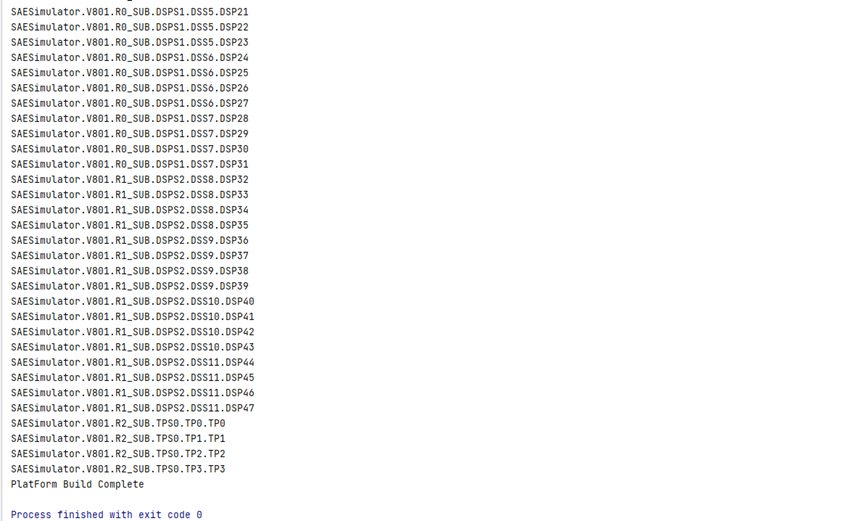
\includegraphics[width=1\textwidth]{硬件平台构建输出消息.png}
    \caption{硬件平台构建输出消息}
    \label{fig:badge}
\end{figure}

\subsection{仿真平台运行模块测试}

仿真平台运行模块功能主要要保证输入的任务用例能够正确的解析任务图信息、调度模块能够按照任务执行
顺序正确读取任务、仿真平台能够将整个任务图按序执行完毕。这些功能将任务图中信息解析出来并由调度
模块读取分配执行,使整个任务用例在仿真平台上完整的运行完毕。同时我们也需要保证任务执行时序以及
关键信息的准确性。仿真平台运行模块的测试结果如表6.5所示:

\begin{table}[]
    \centering\normalsize
    \caption{仿真平台运行模块测试表}
    \begin{tabular}{|c|c|c|c|c|}
    \hline
    \textbf{序号} & \textbf{测试项}                                               & \textbf{操作流程}                                                      & \textbf{预期结果}                                            & \textbf{实际结果} \\ \hline
    1           & \begin{tabular}[c]{@{}c@{}}是否能够完整解析任\\ 务图信息\end{tabular}   & \begin{tabular}[c]{@{}c@{}}运行TaskGraphMgnt\\ 类中Load函数\end{tabular} & \begin{tabular}[c]{@{}c@{}}任务图信息完整包\\ 含在类中\end{tabular}  & 正确            \\ \hline
    2           & \begin{tabular}[c]{@{}c@{}}能否正确按序读取\\ 任务实例\end{tabular}    & \begin{tabular}[c]{@{}c@{}}运行Schedule类中\\ load函数\end{tabular}      & \begin{tabular}[c]{@{}c@{}}将任务图中任务\\ 按序读取\end{tabular}   & 正确            \\ \hline
    3           & \begin{tabular}[c]{@{}c@{}}DMA模块能否正\\ 确执行任务\end{tabular}   & \begin{tabular}[c]{@{}c@{}}发送DMA任务到\\ 硬件模块上执行\end{tabular}         & \begin{tabular}[c]{@{}c@{}}数据能够正确搬\\ 运到相应位置\end{tabular} & 正确            \\ \hline
    4           & \begin{tabular}[c]{@{}c@{}}DSP模块能否正确\\ 执行任务\end{tabular}   & \begin{tabular}[c]{@{}c@{}}发送DSP任务到\\ 硬件模块上执行\end{tabular}         & \begin{tabular}[c]{@{}c@{}}任务执行时延与\\ 任务信息一致\end{tabular} & 正确            \\ \hline
    5           & \begin{tabular}[c]{@{}c@{}}HAC模块能否正确\\ 执行任务\end{tabular}   & \begin{tabular}[c]{@{}c@{}}发送HAC任务到\\ 硬件模块上执行\end{tabular}         & \begin{tabular}[c]{@{}c@{}}任务执行结果与\\ 任务信息一致\end{tabular} & 正确            \\ \hline
    6           & \begin{tabular}[c]{@{}c@{}}仿真平台能否完整\\ 运行整个任务图\end{tabular} & \begin{tabular}[c]{@{}c@{}}运行主函数中的\\ SimRun函数\end{tabular}         & \begin{tabular}[c]{@{}c@{}}任务图中所有任\\ 务正确执行\end{tabular}  & 正确            \\ \hline
    7           & \begin{tabular}[c]{@{}c@{}}仿真运行结果时序\\ 是否正确\end{tabular}    & \begin{tabular}[c]{@{}c@{}}对比数据库仿真信\\ 息与任务用例信息\end{tabular}        & 两者信息一致                                                   & 正确            \\ \hline
    \end{tabular}
    \end{table}

如表6.5我们对仿真平台仿真运行模块进行了测试,测试项1通过运行TaskGraphMgnt模块的Load函数去解析输入的用例文件。最后在调试过程中检测任务图信息是否完整包含在一个Graph类中,测试结果显示任务图信息完整。

测试项2通过运行Schedule类中load函数来读取Graph类中的任务信息,我们通过写测试函数,将任务图信息按序全部打印出来,测试结果显示所有任务按序输出显示在终端上,结果正确。

测试3\textasciitilde 5是为了测试各个硬件模块的功能是否正确。我们通过手动构造各种类型的任务用例到硬件模块的接口FIFO上来模拟调度器模块分配任务的流程,看各个硬件模块能不能正确执行任务用例,且任务执行结果是否和任务描述是否一致。测试结果显示各个硬件模块均能正确执行调度器分配的任务。

测试项6通过运行项目主函数中的SimRun函数运行仿真,函数参数包括任务用例名、任务图执行次数、输出数据库位置、Log文件是否记录等等。我们在硬件平台搭建完成的基础上,使用任务用例输入执行仿真,仿真运行输出信息如图6-2所示。且在数据库中将任务执行信息与任务用例中任务信息相对比,执行时序正确无误。

\begin{figure}
    \centering
    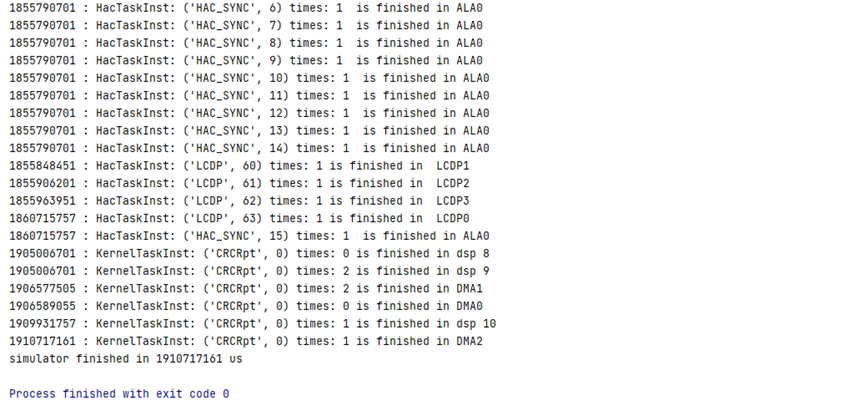
\includegraphics[width=1\textwidth]{仿真运行输出消息.png}
    \caption{仿真运行输出消息}
    \label{fig:badge}
\end{figure}

由上面两个方面的验证能够保证仿真平台的功能的正确性。能够满足业务需求以及后续设计空间探索的需求。

\subsection{仿真平台性能测试}
在对仿真平台功能方面进行测试的同时,我们需要对仿真平台的性能方面进行测试。我们在需求分析阶段提出了几个对于
仿真平台以及设计空间探索流程的性能测试指标,我们针对需求分析中表3-2中指标进行测试,测试结果如
表6.6所示:

\begin{table}[htb]
    \centering\normalsize
    \caption{仿真平台性能测试表}
    \begin{tabular}{|c|c|c|c|l}
    \cline{1-4}
    序号 & 测试项            & 预期结果              & 实际结果   &  \\ \cline{1-4}
    1  & 仿真硬件平台搭建时间     & \textless{}=5s    & 4.76s  &  \\ \cline{1-4}
    2  & 单次单小区仿真执行时间    & \textless{}=15s   & 13.56s &  \\ \cline{1-4}
    3  & 仿真结果时序是否与用例一致  & True              & True   &  \\ \cline{1-4}
    4  & 单次一代遗传算法执行时间   & \textless{}=500ms & 398ms  &  \\ \cline{1-4}
    5  & 设计空间探索结果是否全局最优 & True              & True   &  \\ \cline{1-4}
    \end{tabular}
    \end{table}

如表6.3所示,通过对仿真平台以及设计空间探索流程进行多次运行,得到的测试结果如上表所示。由测试结果
可以看出仿真平台的单次单小区的执行时间低于预期值,满足后续设计空间探索流程的需求。针对需求分析阶段提出的
性能需求的几大指标而言,测试结果都满足性能测试指标需求。

\section{本章小结}

本章主要对仿真平台做了功能上的测试,仿真平台能够正确的构建硬件平台,并能够在硬件平台上运行任务用例,保证任务仿真的时序正确。同时也对设计空间探索的结果进行了分析,并得到了一些结论和在所有目标值方面比较优秀的设计方案。
% !TeX root = ../main.tex

\chapter{结果与展望}

本章主要用来总结本文的工作,总结本文的创新点和不足,并给出在未来工作中的展望
和希望研究的部分。

\section{论文总结}

目前部门内的仿真建模平台是基于SystemC的,模型建模做的十分精密,完全仿真了信
道用例在芯片上的全部执行过程以及在处理器的执行逻辑,但因此整个仿真
平台也十分复杂臃肿,仿真运行比较慢,执行一次用例仿真时间较长。因此,为了解决仿真
时间长和仿真建模繁琐的同时,也为了满足后续设计空间探索的要求,本文设计并实现
了基于SimPy的轻量级仿真平台,并基于轻量级仿真平台打通了设计空间探索流程。

在前期的调研过程中,我们最终确定了以SimPy为仿真环境,以python为开发语言,这样
大大减少了开发时间。以之前基于SystemC的SAE仿真平台各个模块的建模为原型,重新
实现了各个模块的建模。实现了硬件模块建模、硬件平台搭建、用例文件解析、任务调
度以及数据库输出的仿真平台功能。并兼容原有的SAE仿真平台,与原有的仿真平台用例
输入和硬件配置文件输入一致,可以实现一个用例在两个仿真平台上运行,这样了降低
了后续开发人员的工作量。在处理器建模过程中,我们简化了任务在处理器上的执行逻辑,
只对任务的一些关键属性包括触发关系、数据搬运以及执行时延进行仿真。在内存模块建模时
仿真平台并不进行真正的内存开辟和释放,只对内存模块的结构以及执行逻辑进行建模,对相应
的目的内存地址进行标记。这样就极大的优化了仿真平台的执行效率,使得仿真平台能够更加迅速
准确的执行任务用例。

在设计空间探索流程中,我们通过调研现在业内设计空间探索以及多目标优化的案例,
最终确定了以进化算法为设计空间探索的方法。为了简化进化算法的每一代种群的计算
过程,我们采用将仿真过程通过机器学习拟化为一个预测模型,这样将执行一次设计空
间探索流程的时间从4天缩短到2分钟,这样研究人员可以将更多的时间却研究设计空间
探索的结果。

基于以上方面,本文实现的轻量级仿真平台可以实现业务仿真并大大减少了仿真时间,
并在后续一些方案设计中体现了良好的性能。设计空间探索流程的打通为部门内部方案
设计提供了新思路和新方法。

\section{问题和展望}

本文实现的仿真平台虽然能够对比原平台能够实现大部分功能,但调度器部分在原型设
计过程中功能设计比较简单,资源调度方面不够灵活。在硬件模块实现部分,一些具体
的硬件模型没有特例化实现,这些都有待后续完善。

在设计空间探索方面,整个流程虽然打通,但是整个流程的精度并没有很高,只是对现
有的仿真平台做出一个针对性的探索,并没有对更多的平台进行适配,甚至不仅对仿真
平台,还可以对直接从单板上提取的输入输出的格式进行适配。在接下来的完善过程中,
可以改进预测模型的部分,可以通过这方面去适配更多的输入格式,通过调整进化算法
去改善整个设计空间探索流程的精度。



\backmatter
\bibliography{bib/ustc}  % 参考文献使用 BibTeX 编译
% \printbibliography       % 参考文献使用 BibLaTeX 编译

\appendix
% !TeX root = ../main.tex

\chapter{缩略词对照表}
\begin{table}[]
  \normalsize
  \begin{tabular}{p{3cm}p{6cm}l}
  \textbf{缩略词} & \textbf{英文全称} & \textbf{中文对照}   \\
  SoC & System on Chip & 片上系统 \\
  ESL & Electronic System Level & 电子系统级 \\
  RTL & Register transfer Level & 寄存器传输级 \\
  HLS & High Level Synthesis & 高层次综合 \\
  DSE & Design Space Exploratiom & 设计空间探索 \\
  EDA & Electronic Design Automation & 电子设计自动化 \\
  TLM & Transaction Level Modeling & 事务级建模 \\
  MPSoC & Multi-core System on Chip & 片上多处理器系统 \\
  Fifo & first in first out & 先入先出 \\
  DSP & Digital Signal Processing & 数字信号处理 \\
  DMA & Direct Memory Access & 直接存储器访问 \\
  HAC & Hardware Accelerator & 硬件加速器 
  \end{tabular}
  \end{table}
% % !TeX root = ../main.tex

\begin{acknowledgements}

    岁月如梭。转眼,研宄生生涯即将以这篇硕士论文的完成而画上句号。有感时间如白驹过隙,
    却难掩心中的充实与美好。两年半中,母校的师生之情和同学之谊令我永生难忘。
    在此表示由衷的谢意。
    
    首先,我要感谢我的校内指导老师张信明教授。在论文的撰写过程中,张老师始终给予我耐心的
    指导和支持。毕业论文的完成离不开张老师的敦敦教诲。老师对学术要求严谨,同时又平易近人,
    衷心祝愿他永远健康快乐,工作顺利。

    其次,我要感谢华为技术有限公司,给了我实习的机会。使我提前了解到学校与企业的区别,对未来
    的职业发展有了更进一步的认识和思考。同时,我要感谢我的企业导师詹德政,感谢他在工作和生活
    上无私帮助,他在工作上认真严谨的态度、开阔的视野以及丰富的知识深深感染了我。。同时为我的
    论文选题以及工作学习也提供了很多宝贵的建议。其次,我要感谢公司的同事李统学长,他在项目上
    帮助了我很多,不仅为我解决了很多工作中的困惑,还指导我如何提升、快速成长。另外,也要感谢
    同事们和领导在工作上给予的热心指导和无条件信任,使我能更好地融入整个团队,更好地提升技术。

    最后,我要感谢我的朋友和同学,在工作和学习的同时带给我欢乐和帮助。感谢我的父母和家人,感谢他们
    在我身后默默的支持。感谢父母对我的栽培和付出,希望他们永远健康快乐。
    
    \begin{flushright}
        俞思源
    
        二〇二二年五月十一日
    \end{flushright}
\end{acknowledgements}


\end{document}
